\documentclass{vkr}
\usepackage[english, russian]{babel} % переносы
\usepackage{graphicx} % для вставки картинок
\graphicspath{{images/}} % путь к изображениям
\usepackage[hidelinks]{hyperref}
\usepackage{float} % определяет метод H для рисунка с переносом на следующую страницу, ели не помещается
\usepackage{pdflscape}
\addto{\captionsrussian}{\renewcommand{\refname}{СПИСОК ИСПОЛЬЗОВАННЫХ ИСТОЧНИКОВ}}
\usepackage{xltabular} % для вставки таблиц
\usepackage{makecell}
\renewcommand\theadfont{} % шрифт в /thead
\usepackage{array} % для определения новых типов столбцов таблиц
\newcolumntype{T}{>{\centering\arraybackslash}X} % новый тип столбца T - автоматическая ширина столбца с выравниванием по центру
\newcolumntype{R}{>{\raggedleft\arraybackslash}X} % новый тип столбца R - автоматическая ширина столбца с выравниванием по правому краю
\newcolumntype{C}[1]{>{\centering\let\newline\\\arraybackslash\hspace{0pt}}m{#1}} % новый тип столбца C - фиксированная ширина столбца с выравниванием по центру
\newcolumntype{r}[1]{>{\raggedleft\arraybackslash}p{#1}} % новый тип столбца r - фиксированная ширина столбца с выравниванием по правому краю
\newcommand{\centrow}{\centering\arraybackslash} % командой \centrow можно центрировать одну ячейку (заголовок) в столбце типа X или p, оставив в оcтальных ячейках другой тип выравнивания
\newcommand{\finishhead}{\endhead\hline\endlastfoot}
\newcommand{\continuecaption}[1]{\captionsetup{labelformat=empty} \caption[]{#1}\\ \hline }
\usepackage{etoolbox}
\AtBeginEnvironment{xltabular}{\refstepcounter{tablecnt}} % подсчет таблиц xltabular, обычные таблицы подсчитываются в классе

\usepackage[tableposition=top]{caption} % подпись таблицы вверху
\captionsetup{strut=off}
\setlength{\intextsep}{0pt} % Vertical space above & below [h] floats
\setlength{\textfloatsep}{0pt} % Vertical space below (above) [t] ([b]) floats
\DeclareCaptionLabelFormat{gostfigure}{Рисунок #2} %подпись рисунка
\DeclareCaptionLabelFormat{gosttable}{Таблица #2} %подпись таблицы
\DeclareCaptionLabelSeparator{gost}{~--~} %разделитель в рисунках и таблицах
\captionsetup{labelsep=gost}
\captionsetup[figure]{aboveskip=10pt,belowskip=4mm,justification=centering,labelformat=gostfigure} % настройка подписи рисунка
\captionsetup[table]{font={stretch=1.41},skip=0pt,belowskip=0pt,aboveskip=8.5pt,singlelinecheck=off,labelformat=gosttable} % настройка подписи таблицы

\setlength{\LTpre}{8mm} % отступ сверху таблицы
\setlength{\LTpost}{6mm} % отступ снизу таблицы

\usepackage{enumitem}
\setlist{nolistsep,wide=\parindent,itemindent=*} % отступы вокруг списков, выравнивание с учетом разделителя

\usepackage{color} %% это для отображения цвета в коде
\usepackage{listings} %% листинги кода
\setmonofont[Scale=0.7]{Verdana} % моноширный шрифт для листинга

\definecolor{codegreen}{rgb}{0,0.6,0}
\definecolor{codegray}{rgb}{0.5,0.5,0.5}
\definecolor{codepurple}{rgb}{0.58,0,0.82}

\lstset{ %
language=C,                 % выбор языка для подсветки (здесь это С)
numbers=left,               % где поставить нумерацию строк (слева\справа)
numberstyle=\tiny,           % размер шрифта для номеров строк
stepnumber=1,                   % размер шага между двумя номерами строк
numbersep=5pt,                % как далеко отстоят номера строк от подсвечиваемого кода
commentstyle=\color{codegreen},
keywordstyle=\color{magenta},
numberstyle=\tiny\color{codegray},
stringstyle=\color{codepurple},
basicstyle=\linespread{0.95}\ttfamily,
backgroundcolor=\color{white}, % цвет фона подсветки - используем \usepackage{color}
showspaces=false,            % показывать или нет пробелы специальными отступами
showstringspaces=false,      % показывать или нет пробелы в строках
showtabs=false,             % показывать или нет табуляцию в строках
frame=single,              % рисовать рамку вокруг кода
tabsize=2,                 % размер табуляции по умолчанию равен 2 пробелам
captionpos=t,              % позиция заголовка вверху [t] или внизу [b] 
breaklines=true,           % автоматически переносить строки (да\нет)
breakatwhitespace=false, % переносить строки только если есть пробел
escapeinside={\%*}{*)}   % если нужно добавить комментарии в коде
}

\makeatletter % чтобы допускались русские комментарии в листингах
\lst@InputCatcodes
\def\lst@DefEC{%
 \lst@CCECUse \lst@ProcessLetter
  ^^80^^81^^82^^83^^84^^85^^86^^87^^88^^89^^8a^^8b^^8c^^8d^^8e^^8f%
  ^^90^^91^^92^^93^^94^^95^^96^^97^^98^^99^^9a^^9b^^9c^^9d^^9e^^9f%
  ^^a0^^a1^^a2^^a3^^a4^^a5^^a6^^a7^^a8^^a9^^aa^^ab^^ac^^ad^^ae^^af%
  ^^b0^^b1^^b2^^b3^^b4^^b5^^b6^^b7^^b8^^b9^^ba^^bb^^bc^^bd^^be^^bf%
  ^^c0^^c1^^c2^^c3^^c4^^c5^^c6^^c7^^c8^^c9^^ca^^cb^^cc^^cd^^ce^^cf%
  ^^d0^^d1^^d2^^d3^^d4^^d5^^d6^^d7^^d8^^d9^^da^^db^^dc^^dd^^de^^df%
  ^^e0^^e1^^e2^^e3^^e4^^e5^^e6^^e7^^e8^^e9^^ea^^eb^^ec^^ed^^ee^^ef%
  ^^f0^^f1^^f2^^f3^^f4^^f5^^f6^^f7^^f8^^f9^^fa^^fb^^fc^^fd^^fe^^ff%
  ^^^^20ac^^^^0153^^^^0152%
  % Basic Cyrillic alphabet coverage
  ^^^^0410^^^^0411^^^^0412^^^^0413^^^^0414^^^^0415^^^^0416^^^^0417%
  ^^^^0418^^^^0419^^^^041a^^^^041b^^^^041c^^^^041d^^^^041e^^^^041f%
  ^^^^0420^^^^0421^^^^0422^^^^0423^^^^0424^^^^0425^^^^0426^^^^0427%
  ^^^^0428^^^^0429^^^^042a^^^^042b^^^^042c^^^^042d^^^^042e^^^^042f%
  ^^^^0430^^^^0431^^^^0432^^^^0433^^^^0434^^^^0435^^^^0436^^^^0437%
  ^^^^0438^^^^0439^^^^043a^^^^043b^^^^043c^^^^043d^^^^043e^^^^043f%
  ^^^^0440^^^^0441^^^^0442^^^^0443^^^^0444^^^^0445^^^^0446^^^^0447%
  ^^^^0448^^^^0449^^^^044a^^^^044b^^^^044c^^^^044d^^^^044e^^^^044f%
  ^^^^0401^^^^0451%
  %%%
  ^^00}
\lst@RestoreCatcodes
\makeatother
\usepackage{tabularx}

% Режим шаблона (должен быть включен один из трех)
%\ВКРtrue
\Практикаtrue
%\Курсоваяtrue

\newcommand{\Дисциплина}{<<Проектирование и архитектура программных систем>>} % для курсовой
\newcommand{\КодСпециальности}{09.03.04} % Курсовая
\newcommand{\Специальность}{Программная инженерия} % Курсовая
\newcommand{\Тема}{Разработка web-сайта «Русатом – Аддитивные технологии» на платформе} % ВКР Курсовая
\newcommand{\ТемаВтораяСтрока}{1С-Битрикс}
\newcommand{\ГдеПроводитсяПрактика}{ООО <<Мцоб.Онлайн-сервисы>>} % для практики
\newcommand{\РуководительПрактПредпр}{Куркина А. В.} % для практики
\newcommand{\ДолжнРуководительПрактПредпр}{директор} % для практики
\newcommand{\РуководительПрактУнивер}{Чаплыгин А. А.} % для практики
\newcommand{\ДолжнРуководительПрактУнивер}{к.т.н. доцент} % для практики
\newcommand{\Автор}{И. И. Иванов}
\newcommand{\АвторРод}{Иванова И.И.}
\newcommand{\АвторПолностьюРод}{Конева Андрея Вячеславовича} % для практики
\newcommand{\Шифр}{хх-хх-хххх}
\newcommand{\Курс}{4 } % для практики
\newcommand{\Группа}{ПО-11б}
\newcommand{\Руководитель}{А. А. Чаплыгин} % для ВКР и курсовой
\newcommand{\Нормоконтроль}{А. А. Чаплыгин} % для ВКР
\newcommand{\ЗавКаф}{А. В. Малышев} % для ВКР
\newcommand{\ДатаПриказа}{«07» апреля 2023~г.} % для ВКР
\newcommand{\НомерПриказа}{1505-с} % для ВКР
\newcommand{\СрокПредоставления}{«13» июня 2023~г.} % для ВКР, курсового

\begin{document}
\maketitle
\ifПрактика{}\else{
   \newpage
\begin{center}
\large\textbf{Минобрнауки России}

\large\textbf{Юго-Западный государственный университет}
\vskip 1em
\normalsize{Кафедра программной инженерии}
\vskip 1em
\ifВКР{
        \begin{flushright}
        \begin{tabular}{p{.4\textwidth}}
        \centrow УТВЕРЖДАЮ: \\
        \centrow Заведующий кафедрой \\
        \hrulefill \\
        \setarstrut{\footnotesize}
        \centrow\footnotesize{(подпись, инициалы, фамилия)}\\
        \restorearstrut
        «\underline{\hspace{1cm}}»
        \underline{\hspace{3cm}}
        20\underline{\hspace{1cm}} г.\\
        \end{tabular}
        \end{flushright}
        }\fi
\end{center}
\vspace{1em}
  \begin{center}
  \large
\ifВКР{
ЗАДАНИЕ НА ВЫПУСКНУЮ КВАЛИФИКАЦИОННУЮ РАБОТУ
  ПО ПРОГРАММЕ БАКАЛАВРИАТА}
  \else
ЗАДАНИЕ НА КУРСОВУЮ РАБОТУ (ПРОЕКТ)
\fi
\normalsize
  \end{center}
\vspace{1em}
{\parindent0pt
  Студента \АвторРод, шифр\ \Шифр, группа \Группа
  
1. Тема «\Тема\ \ТемаВтораяСтрока»
\ifВКР{
утверждена приказом ректора ЮЗГУ от \ДатаПриказа\ № \НомерПриказа
}\fi.

2. Срок предоставления работы к защите \СрокПредоставления

3. Исходные данные для создания программной системы:

3.1. Перечень решаемых задач:}

\renewcommand\labelenumi{\theenumi)}

\begin{enumerate}
\item проанализировать IT-инфраструктуру предприятия;
\item  разработать концептуальную модель системы управления IT-ин\-фра\-струк\-турой предприятия на основе подхода к управлению и организации ИТ-услуг ITSM;
\item спроектировать программную систему управления IT-ин\-фра\-струк\-турой предприятия;
\item сконструировать и протестировать программную систему управления IT-инфраструктурой предприятия.
\end{enumerate}

{\parindent0pt
  3.2. Входные данные и требуемые результаты для программы:}

\begin{enumerate}
\item Входными данными для программной системы являются: данные
справочников комплектующих, конфигураций, ПО, критериев качества SLA,
ИТ-услуг, департаментов компании; технические данные ИТ-ресурсов; данные входящих заявок на ИТ-ресурсы; данные запросов поставщикам на комплектующие.
\item Выходными данными для программной системы являются: сформированные заявки на обслуживание ИТ-ресурсов; сформированные запросы на
закупку комплектующих; сведения о выполненных работах по заявкам; статусы заявок; выходные отчеты (инфографика) – по качеству услуг, по состоянию ИТ-ресурсов, по деятельности ИТ-отдела, по стоимости обслуживания
ИТ-ресурсов, воронка заявок.
\end{enumerate}

{\parindent0pt

  4. Содержание работы (по разделам):
  
  4.1. Введение.
  
  4.1. Анализ предметной области.
  
4.2. Техническое задание: основание для разработки, назначение разработки,
требования к программной системе, требования к оформлению документации.

4.3. Технический проект: общие сведения о программной системе, проект
данных программной системы, проектирование архитектуры программной системы, проектирование пользовательского интерфейса программной системы.

4.4. Рабочий проект: спецификация компонентов и классов программной системы, тестирование программной системы, сборка компонентов программной системы.

4.5. Заключение.

4.6. Список использованных источников.

5. Перечень графического материала:

\списокПлакатов

\vskip 2em
\begin{tabular}{p{6.8cm}C{3.8cm}C{4.8cm}}
Руководитель \ifВКР{ВКР}\else работы (проекта) \fi & \lhrulefill{\fill} & \fillcenter\Руководитель\\
\setarstrut{\footnotesize}
& \footnotesize{(подпись, дата)} & \footnotesize{(инициалы, фамилия)}\\
\restorearstrut
Задание принял к исполнению & \lhrulefill{\fill} & \fillcenter\Автор\\
\setarstrut{\footnotesize}
& \footnotesize{(подпись, дата)} & \footnotesize{(инициалы, фамилия)}\\
\restorearstrut
\end{tabular}
}

\renewcommand\labelenumi{\theenumi.}

   \abstract{РЕФЕРАТ}

Объем работы равен \formbytotal{lastpage}{страниц}{е}{ам}{ам}. Работа содержит \formbytotal{figurecnt}{иллюстраци}{ю}{и}{й}, \formbytotal{tablecnt}{таблиц}{у}{ы}{}, \arabic{bibcount} библиографических источников и \formbytotal{числоПлакатов}{лист}{}{а}{ов} графического материала. Количество приложений – 2. Графический материал представлен в приложении А. Фрагменты исходного кода представлены в приложении Б.

Перечень ключевых слов: разливы нефти, нейронные сети, мониторинг, спутниковые снимки, распознавание объектов, информационная система, экология, загрязнение водоемов, компьютерное зрение, U-Net, интеллектуальная система, машинное обучение, обработка изображений, предобработка данных, пользовательский интерфейс.

Объектом разработки является система мониторинга водоемов для выявления загрязнений на основе изображений поверхности воды.

Целью выпускной квалификационной работы является разработка интеллектуальной системы распознавания пятен разливов нефти на поверхности водоемов.

В процессе создания системы была разработана архитектура нейронной сети, приложение с графическим интерфейсом для взаимодействия пользователей с системой, сформирован датасет, обучена и протестирована разработанная нейронная сеть.

\selectlanguage{english}
\abstract{ABSTRACT}
  
The volume of work is \formbytotal{lastpage}{page}{}{s}{s}. The work contains \formbytotal{figurecnt}{illustration}{}{s}{s}, \formbytotal{tablecnt}{table}{}{s}{s}, \arabic{bibcount} bibliographic sources and \formbytotal{числоПлакатов}{sheet}{}{s}{s} of graphic material. The number of applications is 2. The graphic material is presented in annex A. The layout of the site, including the connection of components, is presented in annex B.

List of keywords: oil spills, neural networks, monitoring, satellite imagery, object recognition, information system, ecology, water pollution, computer vision, U-Net, intelligent system, machine learning, image processing, data preprocessing, user interface.

The object of the research is the waterbody monitoring system for detectin pollution based on water surface imagery.

The goal of the work is to develop an intelligent system for oil spill detection on the surface of waterbodies.

During the development process, a neural network architecture was designed, a graphical user interface desktop application was developed for user interaction with the system, a dataset was prepared and the developed neural network architecture was trained and tested. 
\selectlanguage{russian}
}\fi
\tableofcontents
%\section*{ОБОЗНАЧЕНИЯ И СОКРАЩЕНИЯ}

ИС -- интеллектуальная система.

ИТ -- информационные технологии. 

ПО -- программное обеспечение.

РП -- рабочий проект.

ТЗ -- техническое задание.

ТП -- технический проект.

НС -- нейронная сеть.

СНС -- сверточная нейронная сеть.

U-Net -- архитектура нейронной сети для сегментации изображений.

CUDA -- технология параллельных вычислений NVIDIA.

UML (Unified Modelling Language) -- язык графического описания для объектного моделирования в области разработки программного обеспечения.

\ifПрактика{}\else{\section*{ВВЕДЕНИЕ}
\addcontentsline{toc}{section}{ВВЕДЕНИЕ}

Аддитивные технологии (АТ) начали активно развиваться со времени получения первых трехмерных изображений изделий на дисплеях компьютеров. Начало положила стереолитография, затем довольно многочисленные новые принципы стали называть технологиями быстрого прототипирования, затем укоренилось название "<Аддитивные технологии">. Интенсивность развития данных технологий не имеет аналогов. АТ изменили процессы проектирования и конструирования изделий, превратив их в процессы непрерывного создания изделий. Современные проектирование и производство изделий невозможно представить без данного рода технологий. 3D-принтеры стали такими же распространенными, как и персональные компьютеры. С помощью 3D-принтеров получают ткани, обувь, продукты питания, а также выращивают человеческие органы. Во многих отраслях, например, в космической отрасли, альтернативы аддитивным технологиям нет.

АТ предполагают изготовление детали методом послойного нанесения материала, в отличие от традиционных методов формирования детали, за счёт удаления материала из массива заготовки.

При использовании АТ все стадии реализации проекта от идеи до материализации находятся в единой технологической цепи, в которой каждая технологическая операция выполняется в цифровой CAD/CAM/CAE-системе.

Современные компании, видя, как развиваются информационные технологии, пытаются использовать их выгодно для своего бизнеса, поэтому запускают свой web-сайт. С его помощью предприятие может заявить о себе, проинформировать потенциального заказчика об услугах или продуктах, которые предоставляет, а также позволяет пользователям сделать с помощью сайта онлайн-заказ, произвести покупку или оплатить счета.

Сайт считается лицом компании и может существенно повысить ее имидж. Любой пользователь сети Интернет сможет получить необходимую информацию о компании в любой момент, появляется возможность найти контактные телефоны, адрес и e-mail, чтобы связаться с компанией. Сейчас большинство клиентов узнают о ее существовании именно через сайт. Поэтому сайт можно назвать самой лучшей рекламой. 

Главной задачей профессионально построенного сайта является превращение посетителя, зашедшего на сайт, в потенциального клиента.

\emph{Цель настоящей работы} – разработка web-сайта компании для привлечения новой аудитории, увеличения заказов, рекламы продукции и услуг компании. Для достижения поставленной цели необходимо решить \emph{следующие задачи:}
\begin{itemize}
\item провести анализ предметной области;
\item разработать концептуальную модель web-сайта;
\item спроектировать web-сайт;
\item реализовать сайт средствами web-технологий.
\end{itemize}

\emph{Структура и объем работы.} Отчет состоит из введения, 4 разделов основной части, заключения, списка использованных источников, 2 приложений. Текст выпускной квалификационной работы равен \formbytotal{lastpage}{страниц}{е}{ам}{ам}.

\emph{Во введении} сформулирована цель работы, поставлены задачи разработки, описана структура работы, приведено краткое содержание каждого из разделов.

\emph{В первом разделе} на стадии описания технической характеристики предметной области приводится сбор информации о деятельности компании, для которой осуществляется разработка сайта.

\emph{Во втором разделе} на стадии технического задания приводятся требования к разрабатываемому сайту.

\emph{В третьем разделе} на стадии технического проектирования представлены проектные решения для web-сайта.

\emph{В четвертом разделе} приводится список классов и их методов, использованных при разработке сайта, производится тестирование разработанного сайта.

В заключении излагаются основные результаты работы, полученные в ходе разработки.

В приложении А представлен графический материал.
В приложении Б представлены фрагменты исходного кода. 
}\fi
\section{Анализ предметной области}
%Тема - Интеллектуальная система мониторинга и распознавания загрязнений водоемов
%написать про методы распознавания разливов иишками, их плюсы и минусы
%примерная структура - разливы, способы мониторинга, нейронки (и их исследование)

\subsection{Нефтяные разливы}

\subsubsection{Экологическая опасность нефтяных разливов}
%частота разливов, крупные трагедии, причины разливов (то есть не только транспорт)
Разлив нефти -- аварийный выброс нефти или нефтепродуктов в окружающую среду. Нефтяные разливы происходят с высокой частотой и являются серьезной проблемой нефтегазовой отрасли. Каждый разлив приводит к масштабным последствиям для окружающей среды и требует значительных финансовых затрат для устранения самого разлива и минимизации экологического ущерба. 

Ярким примером является инцидент на буровой платформе Deepwater Horizon, принадлежавшей британской нефтегазовой компании British Petrolium. 20 апреля 2010 года, в результате нарушения технологических норм цементирования скважины, произошел взрыв, который привел к гибели 11 человек и неконтролируемому выбросу нефти в Мексиканский залив на протяжении нескольких месяцев. В окружающую среду попало около 400 тысяч тонн нефти. Эта катастрофа, ставшая крупнейшим в истории США разливом нефти, привела к массовой гибели животных, таких как дельфины, морские черепахи, тем самым нанеся колоссальный ущерб морским экосистемам, по некоторым оценкам сохраняющийся и по сей день. Расходы на ликвидацию происшествия, а также затраты на штрафы и компенсации, составили около 65 миллиардов долларов.

16 марта 1978 года французский супертанкер Amoco Cadiz, попав в шторм, потерял управление и разбился о скалы у берегов французского региона Бретань. Это происшествие привело к выбросу 220 тысяч тонн сырой нефти в Атлантический океан, загрязнив более 300 километров французского побережья. Пролившаяся нефть образовала пятно протяженностью 19 километров и поникла в песок на глубину до 50 сантиметров, образовав асфальтоподобные корки, сохранявшиеся на протяжении нескольких лет. В защищенных от волн районах нефть сохранялась до 10 лет, тем самым замедляя восстановление экосистемы, понесшей масштабный ущерб -- загрязнение вызвало гибель около 20 тысяч птиц, множества донных организмов, таких как моллюски и ракообразные. Рыбаки сообщали о сокращении уловов в два раза, а сама рыба нередко имела различные язвы и опухоли. Компания Amoco, владелец танкера, выплатила Франции компенсацию в размере 230 миллионов долларов.

Не менее разрушительными оказались последствия крушения танкера Prestige, затонувшего в ноябре 2002 года. Получив повреждения у побережья Испании, корпус судна раскололся, что привело к попаданию примерно 60 тысяч тонн нефти в Атлантический океан. Растянувшееся на более чем 2000 километров вдоль побережья Галисии нефтяное пятно поставило под угрозу существование 25 охраняемых видов животных, уничтожило популяции рыб, кораллов, моллюсков. Согласно государственной оценке, зачистка побережья Галисии обошлась в 2,5 миллиарда евро, а нанесенный ущерб составил 368 миллионов евро. 

В июле 2010 года нефтепровод, принадлежащий американской корпорации Enbridge, разорвало в результате коррозии трубы, что послужило причиной попадания более 2,7 тонн битумной нефти в реку Каламазу, пролившейся на 40 километров по руслу реки и осевшей на дне. Осевшая нефть отравила донные отложения реки, что привело к массовой гибели рыб, популяции которых начали возвращаться только спустя 10 лет. Кроме того, токсины сделали речную воду непригодной для питья, а из-за ядовитых испарений нефти некоторые жители близлежащих районов жаловались на головные боли и тошноту.  Поскольку убирать пролившуюся нефть пришлось не только с поверхности, но и со дна реки, очистные мероприятия были значительно затруднены, что повысило стоимость их проведения -- она составила примерно 1,2 миллиарда долларов.

Утром 15 декабря 2024 года в Керченском проливе в результате шторма танкеры <<Волгонефть-212>> и <<Волгонефть-239>>, перевозившие в общей сложности около 9000 тонн мазута, потерпели крушение. По различным оценкам в море попало от 2,5 до 5 тысяч тонн мазута, разлившегося по площади более 400 м$^{2} $. Загрязнение затронуло около 70 километров береговой линии и привело к гибели более 200 птиц и 70 дельфинов, среди которых были охраняемые виды. Реагируя на происшествие, власти вели режим чрезвычайной ситуации на федеральном уровне и объявили о начале масштабных очистных работ с участием 300 человек и 60 единиц специальной техники, продолжающихся по сей день.

Вследствие принятия множества международных законов и соглашений, совершенствования технологических процессов можно отметить уменьшение частоты крупных происшествий, приводящих к масштабным разливам нефти. Однако, некоторые исследования\cite{spill_db} отмечают, что информация о разливах нефти не всегда достоверна, утверждая, что многие менее крупные инциденты никогда не попадают в поле зрения государственных служб контроля и СМИ, что приводит к отсутствию данных об этих инцидентах в международных и государственных базах. 

\subsubsection{Причины и источники загрязнений}
Основными источниками разливов нефти являются различные утечки на этапах добычи, хранения и транспортировки нефти и нефтепродуктов. Причинами возникновения утечек могут являться как стихийные бедствия, такие как штормы, землетрясения и эрозия, так и техногенные факторы, включая отказы оборудования, человеческие ошибки.  В таблице 1.1 указаны основные источники попадания нефти в мировой океан\cite{spill_reasons}.

\begin{xltabular}{\textwidth}{|X|>{\setlength{\baselineskip}{0.7\baselineskip}}p{4cm}|}
	\caption{Основные источники попадания нефти в мировой океан\label{oil_source:table}}\\
	\hline 
	\centrow Источник & 
	\centrow млн. т/год \\ 
	\hline 
	\endfirsthead
	
	\caption*{Продолжение таблицы \ref{oil_source:table}}\\
	\hline 
	\centrow Источник & 
	\centrow млн. т/год \\ 
	\hline 
	\endhead
	
	Морская транспортировка (кроме аварийных разливов) & 1{,}83 \\ \hline
	Аварийные разливы & 0{,}3 \\ \hline
	Речной сток, включая сточные воды городов & 1{,}9 \\ \hline
	Сточные воды прибрежной зоны & 0{,}8 \\ \hline
	Естественные нефтяные скважины & 0{,}6 \\ \hline
	Добыча нефти в море & 0{,}08 \\ \hline
	\textbf{Всего} & \textbf{5{,}51} \\ \hline
\end{xltabular}



Наиболее часто разливы нефти появляются в результате аварии на танкере, перевозящем нефть или нефтепродукты. Среди причин возникновения таких аварий можно выделить столкновения, посадки на мель, штормовые повреждения, нарушение герметичности резервуаров. Эти происшествия нередко приводят к масштабным выбросам нефти в морскую или речную среду, при этом загрязняя не только воду, но и зачастую прибрежные зоны, в районе которых произошла авария.
 
Морская добыча нефти проводится с помощью масштабных комплексов, использующих комплекс инженерно-технических решений. Такие происшествия, как повреждения герметизации скважин, отказ оборудования, ошибки при цементировании или нарушения технологических регламентов приводят к выбросам добываемой нефти из подземных резервуаров, что в свою очередь приводит к разливам, плохо поддающимся локализации.

Трубопроводы, используемые для транспортировки нефти на большие расстояния, могут дать течь вследствие коррозии труб, механических повреждений, ошибок в обслуживании. В результате в воде может образоваться нефтяной разлив, который может долго оставаться незамеченным, если трубопровод проходит под водой. Кроме того, серьезную угрозу загрязнения представляет преднамеренное разрушение нефтяной инфраструктуры, особенно в зонах активных боевых действий. Атаки на эти объекты не только приводят к масштабным утечкам, но и затрудняют обнаружение и ликвидацию последствий разливов.

Промышленные предприятия, связанные с переработкой нефти, могут сбрасывать загрязненные нефтью или продуктами ее переработки воды в близлежащие водоемы. Наряду с этим отходы ремонтных мастерских, автозаправочных станций также могут попадать в водоемы, что приводит к еще большему загрязнению.

Нефтяные утечки происходят не только по вине человека, но и в ходе естественного просачивания из нефтеносных пластов земли через трещины в коре. Чаще всего это происходит в районах активной геологической активности. Несмотря на относительно незначительные объемы, эти утечки также оказывают негативное влияние на экосистемы.

\subsection{Методы мониторинга разливов нефти}

Своевременное обнаружение и ликвидация нефтяных разливов -- ключевые задачи для сохранения экологической безопасности водоемов. В связи с этим широко распространены различные виды мониторинга состояния водоемов. среди которых выделяются визуальные методы наблюдения за поверхностью воды. В отличие от лабораторных исследований, визуальное исследование позволяет намного быстрее охватить большие территории и не требует физического контакта с объектом, что позволяет оперативно обнаружить новые разливы нефти, особенно в труднодоступных акваториях. 

Одним из самых распространенных методов визуального мониторинга является спутниковая съемка. Современные спутники, оснащенные высокоточными сенсорами, позволяют получить качественные снимки поверхности воды и хорошо отображают аномалии, такие как нефтяные пятна. Спутниковая съемка охватывает сотни квадратных километров поверхности Земли в одном снимке, а использование групп спутников позволяет получать новые данные с высокой периодичностью. Кроме того, использование многих спутников бесплатно, а данные размещены в открытом доступе, что снижает стоимость процедур мониторинга. Однако, зависимость космической съемки от погодных условий и времени суток значительно осложняет наблюдение за поверхностью водоемов и является существенным недостатком этого метода.

В условиях плохой видимости, ограничивающих работу спутников, применяются радиолокационные спутниковые снимки. В отличие от оптических сенсоров, радары полагаются на электромагнитные сигналы и фиксирую отраженный поверхностью воды отклик, что и позволяет вести съемку в любую погоду и время суток. На радарных снимках нефтяные пятна обычно проявляются в качестве темных областей, что повышает их информативность в задачах обнаружения нефтяных пятен и пленок.  Так, исследование радиолокационных снимков Керченского пролива с использованием спутников Sentinel-1A/B за период с 2017 по 2021 годы показало высокую точность этого метода и позволило исследовать частоту появления, масштаб нефтяных разливов и их источники на основании 2597 пятен, появившихся на снимках за этот период\cite{radiophoto}. Несмотря на гибкость этого метода, полученные снимки нередко проявляют сторонние объекты, например различные биологические образования, создавая визуально похожие участки на изображениях. Наличие таких ложных данных требует участия эксперта, отличающего действительные нефтяные пятна от схожих объектов, в процессе мониторинга. Кроме того, радиолокационные изображения значительно дороже, что еще больше повышает стоимость мониторинга.

Наконец, высокую эффективность показал метод аэросъемки поверхностей воды. Вместе с развитием беспилотных летательных аппаратов, или БПЛА, наблюдение за водоемами с малой высоты стало высокоэффективным и экономически оправданным методом мониторинга. БПЛА часто оснащаются камерами высокого разрешения, что позволяет получать самые качественные снимки из перечисленных методов, а высокая степень гибкости в построении маршрутов и простота управления делают этот метод самым доступным. Недостатками аэросъемки с помощью БПЛА являются ограниченность радиуса и времени полета, что делает его малоэффективным для мониторинга больших поверхностей воды, таких как моря. Беспилотные аппараты часто используются в составе систем мониторинга вместе с спутниковыми системами для уточняющих съемок в определенных секторах, снимки которых получены из космоса. 

Перечисленные выше дистанционные методы используются для получения визуальных данных, являющихся источником информации для обнаружения нефтяных разливов. Чтобы обнаружить загрязнение, необходимо проанализировать полученные данные. Учитывая высокое количество изображений, полученных для анализа, этот процесс занимает значительное время. Более того, если изображения получаются в режиме реального времени, например в формате видеосъемки, то для обнаружения разлива нефти необходимо постоянное присутствие наблюдателя. В настоящее время для задач анализа изображений все чаще используются нейронные сети.

\subsection{Нейронные сети}
 
 \subsubsection{История появления нейронных сетей}
 
 Идеи, которые легли в основу современных нейронных сетей, берут свое начало в философии и математике, а основные принципы исследовались задолго до появления вычислительных систем как таковых. Правила, руководящие рациональной частью мышления были сформированы Аристотелем в далеких 384 -- 322 годах до нашей эры. Впоследствии формальные правила рассуждений и процессы мышления стали предметом исследований не менее известных философов, среди которых были Томас Гоббс (1588-1679),  Рене Декарт (1596-1650) и Рудольф Карнап (1891-1970)\cite{nn_history}. Известные математики, такие как Джордж Буль (1815-1864) и Готтлоб Фреге (1848-1925), внесли вклад в разработку логических систем, впоследствии ставших источниками исследований моделирования искусственного интеллекта. 
 
 Первая модель искусственного нейрона была предложена Уорреном МакКаллоком и Уолтером Питтсом в 1943 году. Модель представленного ими логического устройства показана на рисунке~\ref{fig:neuron}.
 
 \begin{figure}[h]
	\centering
	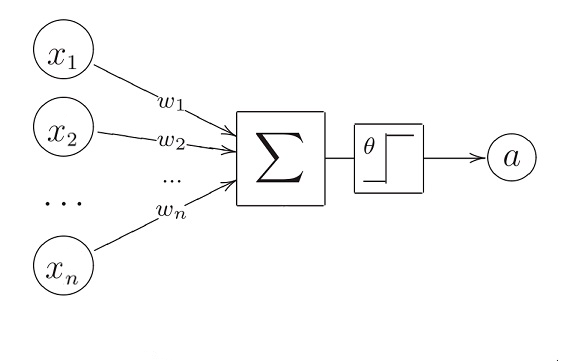
\includegraphics[width=0.7\linewidth]{images/neuron}
	\caption[]{Искусственный нейрон}
	\label{fig:neuron}
\end{figure}

Модель состоит из входов x$_{1}$, x$_{2}$, ... , x$_{n}$, весов w$_{1}$, w$_{2}$, ... , w$_{n}$, сумматора и функции активации. Попадая на входы, каждое значение x$_{i}$ умножается на значение соответствующего веса w$_{i}$, обозначающего его важность, после чего поступает на сумматор, вычисляющий сумму всех поступивших на него сигналов:
\[
z = w_1 x_1 + w_2 x_2 + \cdots + w_n x_n
\]
Полученная сумма затем сравнивается с пороговым значением θ. Если сумма больше, то нейрон возбуждается (выходное значение а = 1), в противном случае остается в состоянии покоя (выходное значение а = 0). Данная модель может выполнять только бинарные операции, получая на вход значения 0 и 1, требует ручного задания весов, также являющихся бинарными, и порогового значения, что значительно ограничивает её возможности. 

Несмотря на ограничения, предложенный МакКаллоком и Питтсем искусственный нейрон показал способность выполнять базовые логические операции, такие как И, ИЛИ и НЕ. Эта модель стала основой для дальнейшей теории нейронных вычислений, а все современные нейронные сети состоят из доработанных версий оригинальных нейронов. 

 Спустя несколько лет идеи, взяв за основу исследования МакКаллока и Питтса, американский ученый Фрэнк Розенблатт предложил схему перцептрона - устройства, моделирующего восприятие информации головным мозгом человека. Перцептрон состоит из входных датчиков, ассоциативных и реагирующих элементов\cite{perceptron}. Схема простейшего перцептрона показана на рисунке~\ref{fig:simpleperceptron}.
 
\begin{figure}[h]
	\centering
	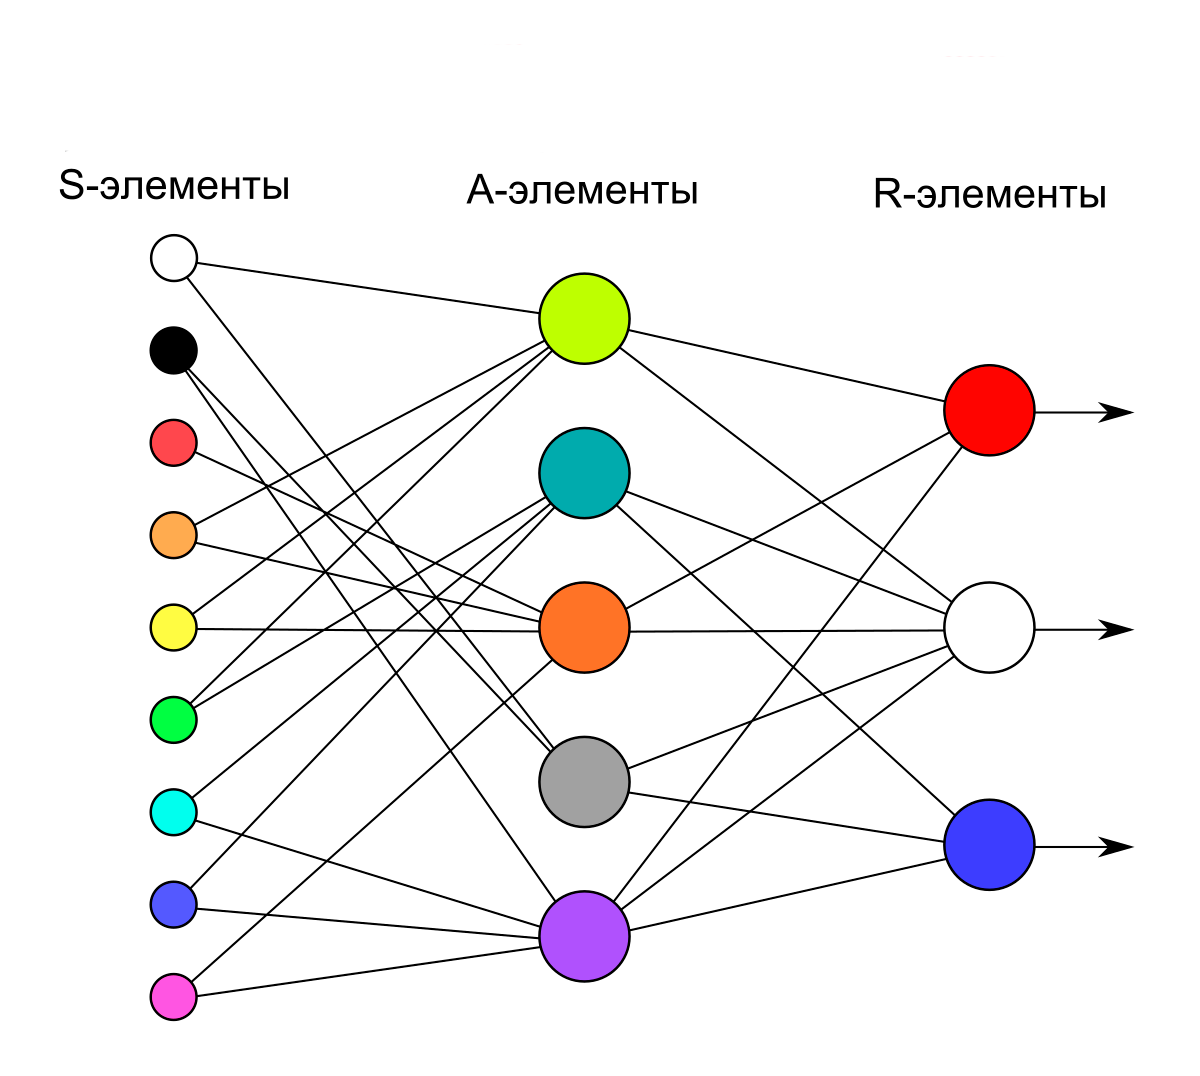
\includegraphics[width=0.7\linewidth]{images/Simple_perceptron}
	\caption{Схема однослойного перцептрона}
	\label{fig:simpleperceptron}
\end{figure}
 
 Однослойный перцептрон подходит для решения задачи классификации данных. Для обучения задаются не только входные значения, но и известные ожидаемые результаты. Как и в случае работы нейрона МакКаллока - Питтса, входные значения (S-слой) передаются на ассоциативные элементы (А-слой), где вычисляется взвешенная сумма поступивших сигналов, являющихся произведениями входных значений и весов связей и, наконец, если сумма превышает заданный порог θ, то результат подается на реагирующий элемент (R-слой). Если выходное значение не совпадает с ожидаемым, то веса связей S--A модифицируются по формуле:
 \[
 w_{ij}(t+1) = w_{ij}(t) + \eta \cdot \delta \cdot X_{j},
 \]
 где t и t$_{1}$ -- номера текущей и следующей итераций процесса, $\eta$ -- коэффициент обучения, находящийся в диапазоне 0<$\eta$<1, $\delta$ -- разность между ожидаемым и полученным значением, i и j -- номера входа и нейрона в слое соответственно, после чего перцептрон заново обрабатывает входные значения до тех пор, пока все выходные значения не совпадут с ожидаемыми. 
 
 Однако, несмотря на успехи в исследованиях, дальнейшее изучение нейронных сетей столкнулось с скептицизмом. Основной причиной стала невозможность однослойных сетей решать многие простые задачи, среди которых операция <<исключающего ИЛИ>>. Формальное доказательство невозможности решения нелинейных задач однослойным перцептроном было предоставлено Марвином Минским и Сеймуром Папертом в книге <<Перцептроны>>, выпущенной в 1969 году. 
 
 После выхода книги, исследовательский интерес к области нейронных систем значительно упал, но не исчез полностью. В 1970-х активно проводились исследования многослойных перцептронов, был разработан алгоритм обратного распространения ошибки для их обучения, позволяющий преодолеть многие ограничения, обозначенные в работе <<Перцептроны>>, но впоследствии оказавшийся не универсальным. Также разрабатывались альтернативные модели нейронных сетей, такие как когнитрон, предложенная Кунихико Фукусимой в 1975 году, ставшая первой моделью, реализующей обучение без учителя. Основной идеей когнитрона является чередование возбуждающих и подавляющих слоев, что позволяет извлекать отдельные признаки и обобщать изображения. Обучение без учителя основано на конкуренции между нейронами -- чем сильнее конкретный вход, тем больший вес ему присваивается, что приводит к заглушению соседних нейронов в конкретном слое. Через пять лет Фукусима представил доработанную и более устойчивую версию когнитрона -- неокогнитрон, состоящий из чередующихся слоев S-элементов, отвечающих за выделение признаков, и C-элементов, подавляющих искажения. Когнитрон и неокогнитрон эффективны для решения задач распознавания образов и стал основой для современных сверточных нейронных сетей. 
 
 Ключевым моментом развития нейронных сетей явилась разработка метода обратного распространения ошибки. Впервые этот метод был описан в 1974 году Александром Галушкиным и Полом Вербосом, одновременно и независимо сформулировавшим его, и формализован в 1986 году Дэвидом Румельхартом, Джеффри Хинтоном и Рональдом Уильямсом. Основной идеей стало распространение ошибки в обратном прямому распространению сигналов направлении. Метод реализует вычисление градиента ошибки по каждому весу нейрона в сети, начиная с выходного слоя и двигаясь к входному, что позволяет корректировать веса для минимизации ошибки предсказания. Появление обратного распространения предоставляет возможность обучения многослойных нейронных сетей на сложных зависимостях и выполнять более точную классификацию.
 
 \subsubsection{Современные типы нейронных сетей}
 
 В настоящее время нейронные сети являются эффективными инструментами машинного обучения, успешно применяемые в широком спектре задач\cite{haikin_neural}. На сегодняшний день разработано большое количество различных архитектур нейронных сетей, обладающих уникальными свойствами и наиболее подходящих для реализации конкретных задач.
 
 Многослойный перцептрон, также известный как сеть прямого распространения, является базовой архитектурой полносвязной нейронной сети. Многослойный перцептрон состоит из входного слоя, одного или нескольких скрытых слоев и выходного слоя, причем каждый элемент конкретного слоя связан со всеми элементами следующего за ним слоя.
 
\begin{figure}[h]
	\centering
	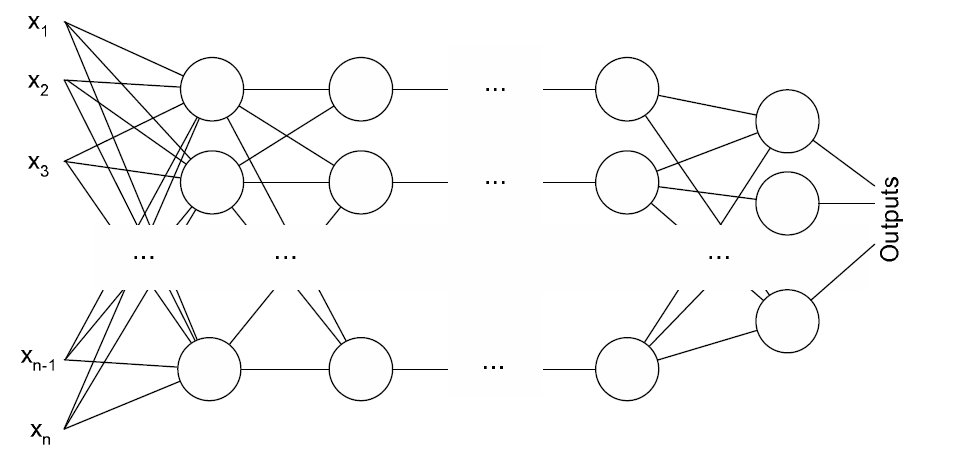
\includegraphics[width=0.7\linewidth]{images/MLP}
	\caption{Многослойный перцептрон}
	\label{fig:mlp}
\end{figure}

Во время обработки информации данные последовательно передаются от входа к выходу без использования сторонних циклов или обратной связи. Обучение полносвязных сетей выполняется при помощи алгоритма обратного распространения ошибки, используемого вместе с параллельным спуском.  Эти нейронные сети позволяют аппроксимировать и приближать практически любые непрерывные функции. Недостатками данной модели является плохая масштабируемость на задачи с большими входными данными, а также большие временные затраты на обучение, что делает ее непригодной для работы с изображениями.

Рекуррентная нейронная сеть разработана для работы с последовательными данными, например текстом, аудиосигналами\cite{rostovtsev_neural}. Отличительной чертой этого типа является наличие внутренней памяти, позволяющей учитывать контекст предыдущих вычислений при обработке новых данных. Базовой архитектурой рекуррентной сети является сеть входных, скрытых и выходных узлов, каждый из которых соединен с остальными. На вход каждого шага вместе с входными данными подается результат обработки предыдущего шага, что позволяет моделировать временные зависимости. В рамках этого подхода следует отметить, что в процессе обработки данных могут возникать проблемы с исчезновением или резким увеличением градиента ошибки. Эти недостатки могут быть устранены в процессе разработки усовершенствованной сети с долгой краткосрочной памятью, LTSM. LTSM является сетью с ячейками памяти, позволяющими сохранять информацию на длительные промежутки времени. Обычно формируется с использованием <<вентилей>>, использующихся для контроля информации на входах и выходах памяти блоков.

\begin{figure}[h]
	\centering
	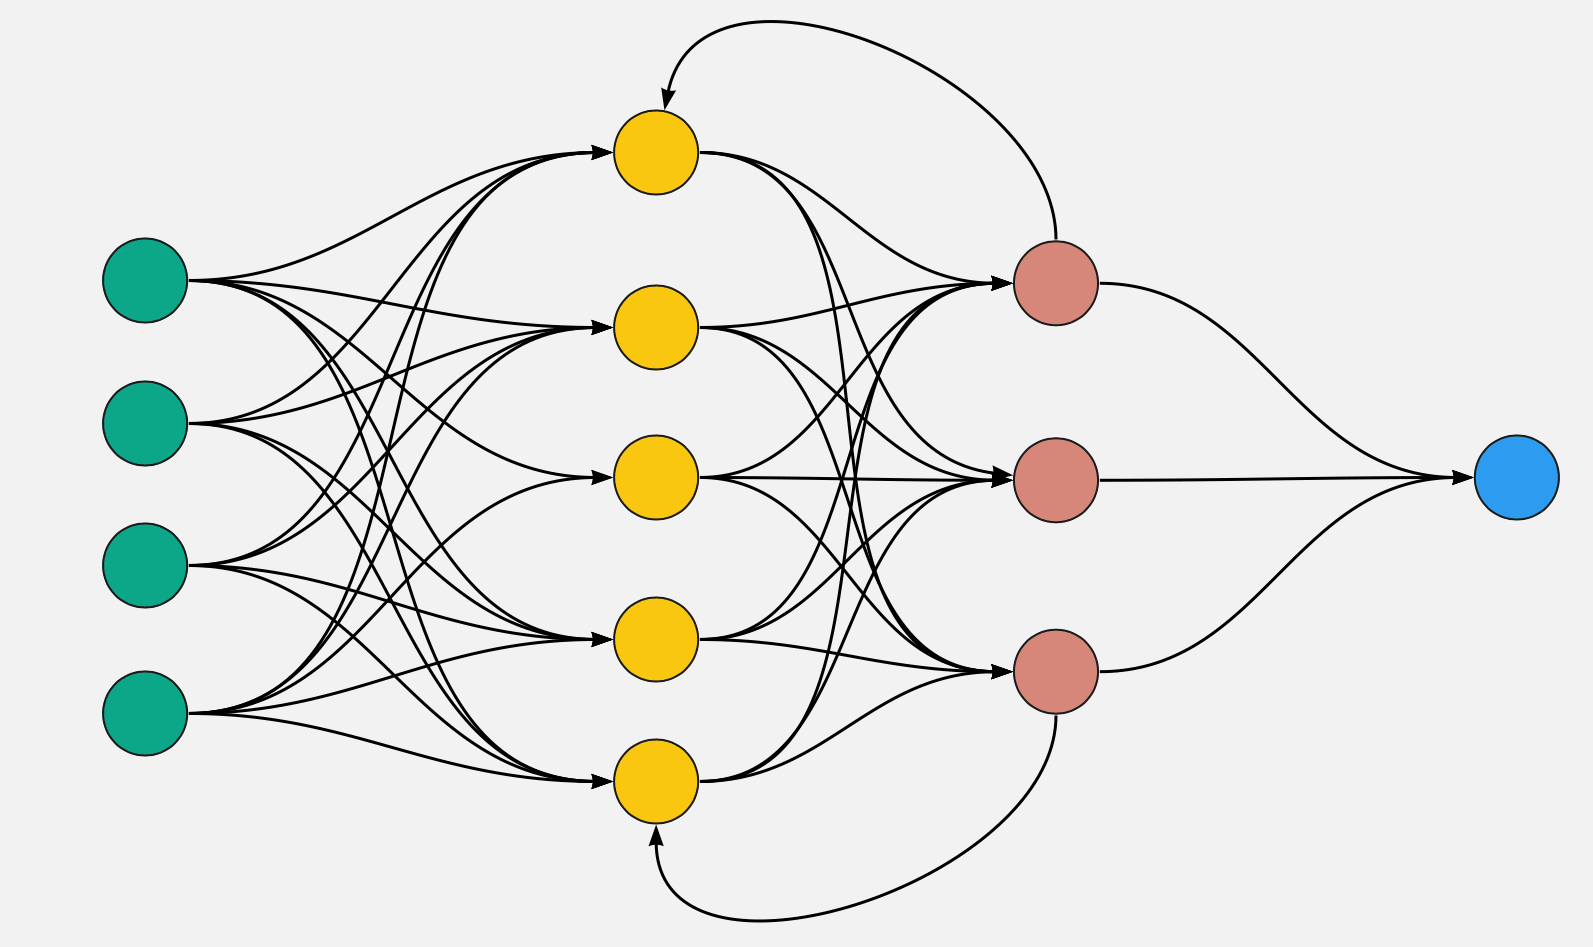
\includegraphics[width=0.7\linewidth]{images/RNN}
	\caption{Рекуррентная нейронная сеть}
	\label{fig:rnn}
\end{figure}

\subsubsection{Сверточные нейронные сети}

Сверточная нейронная сеть (СНС) -- особый класс многослойных перцептронов, разработанный с целью распознавания образов\cite{bychkov_cnn}. Существенным моментом, определяющим практическую эффективность, является то, что СНС обладают высокой степенью инвариантности к пространственным искажениям, таким как смещения и повороты. На рисунке~\ref{fig:cnn} приведена типовая архитектура СНС.

\begin{figure}[h]
	\centering
	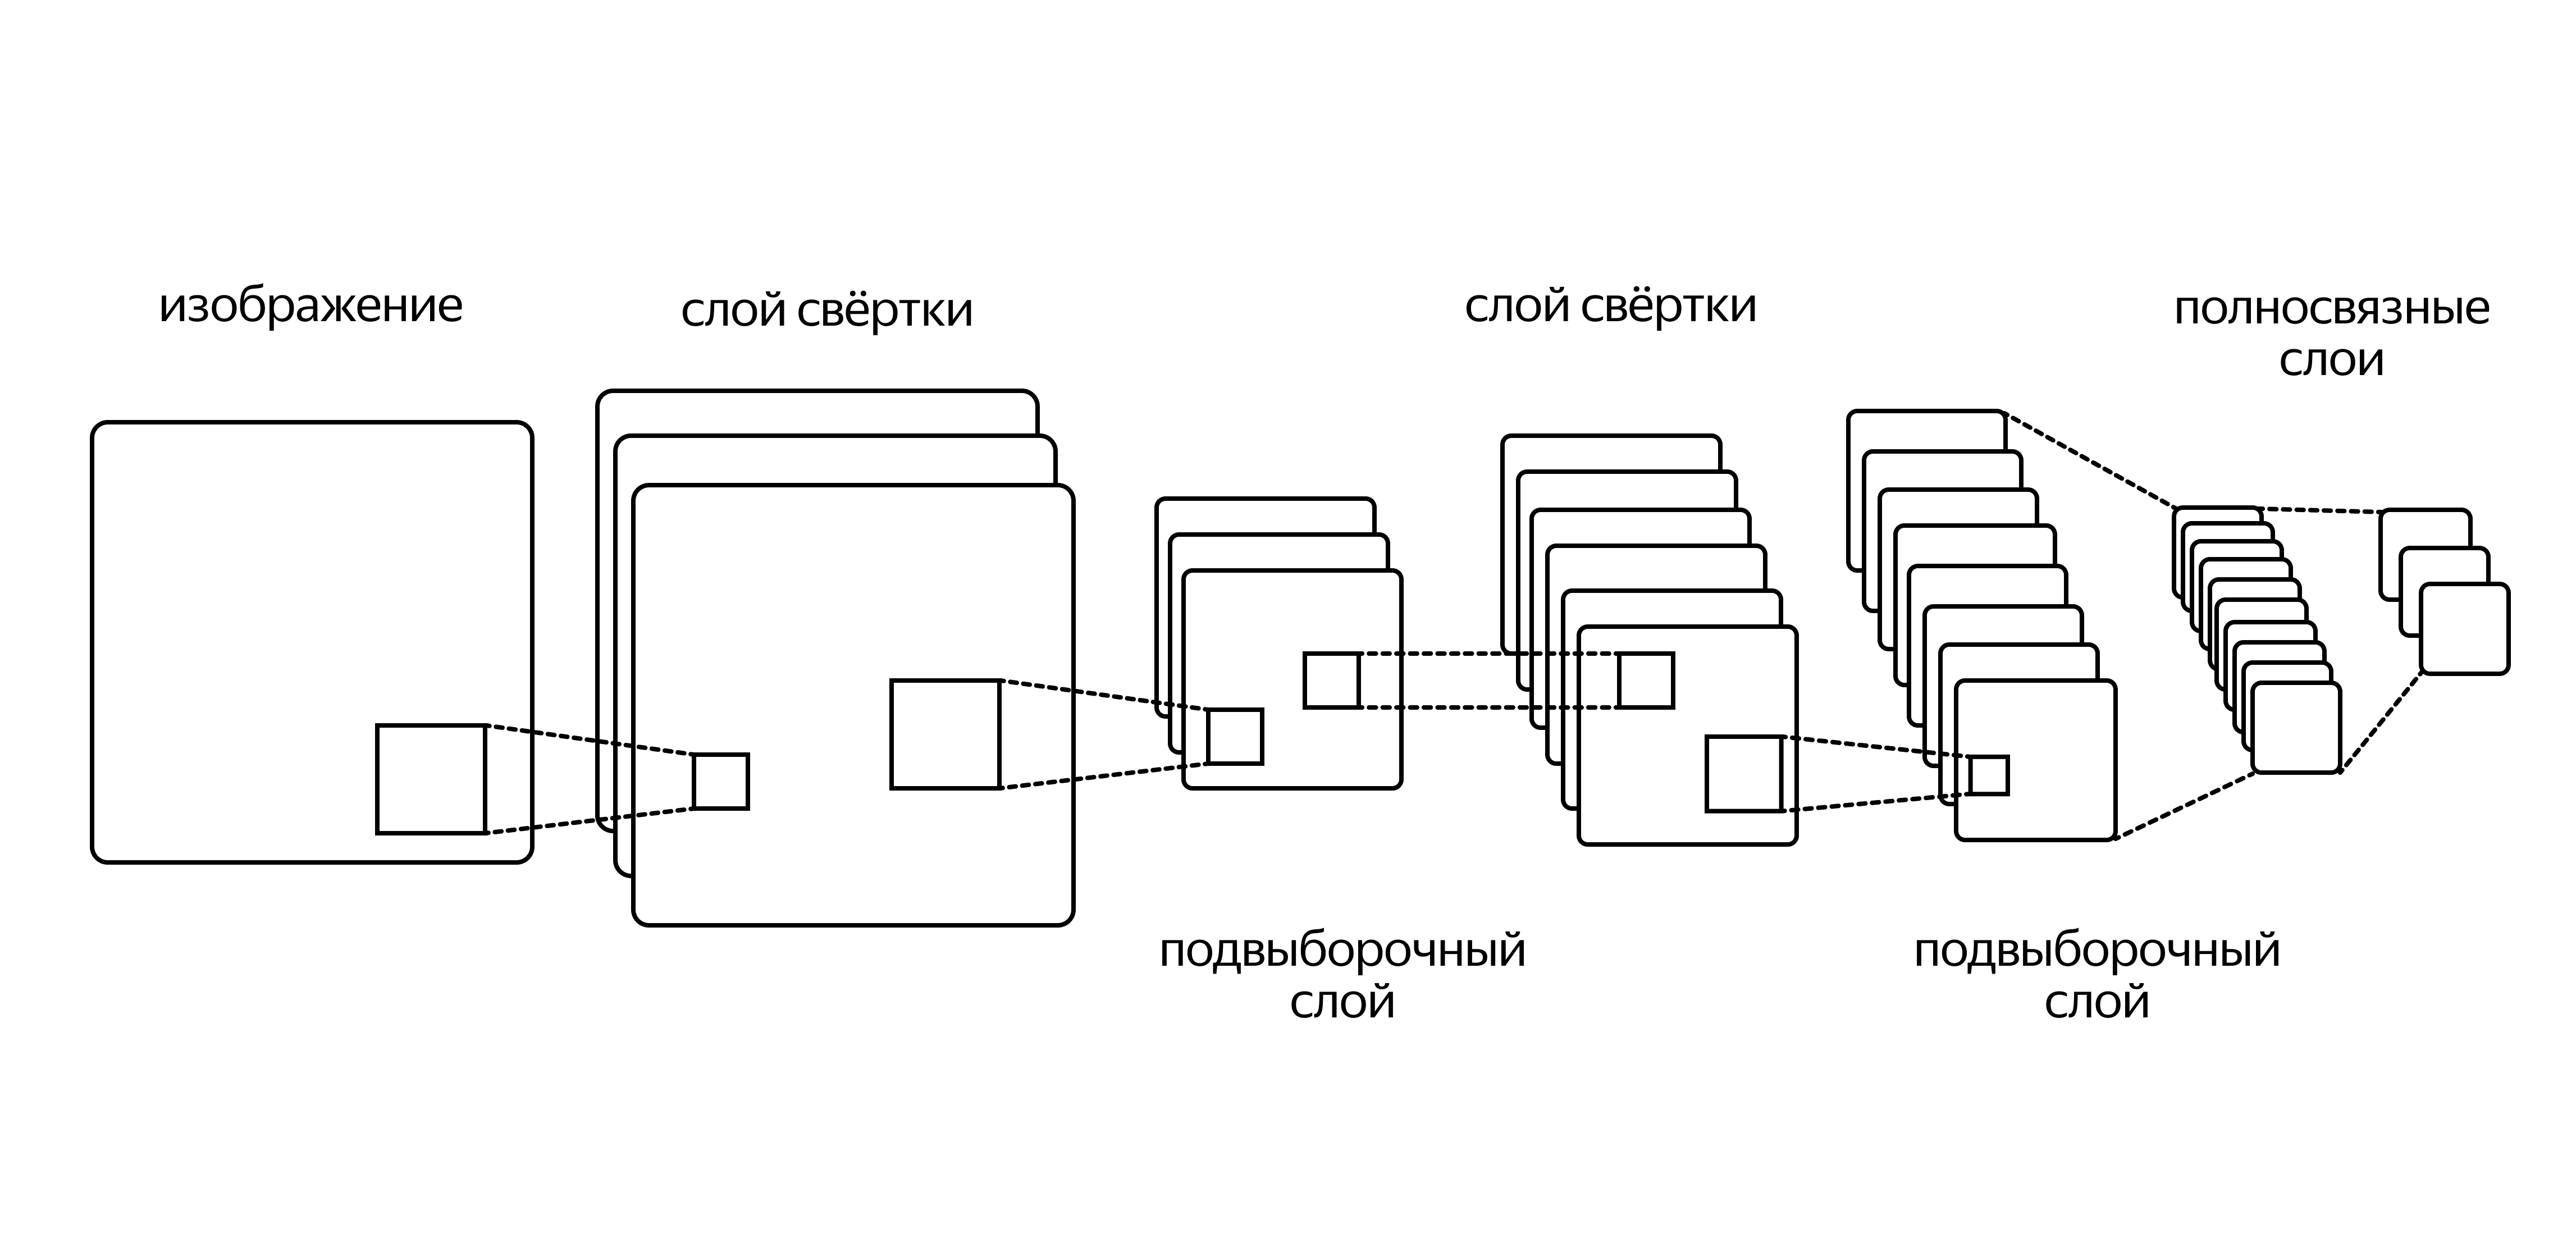
\includegraphics[width=0.7\linewidth]{images/CNN}
	\caption{Архитектура сверточной нейронной сети}
	\label{fig:cnn}
\end{figure}

Сверточные нейронные сети работают с изображениями, представленными в виде тензоров -- трехмерных массивов чисел или массивов матриц чисел. Для моделирования и отображения подобной информации следует учитывать формат представления изображений в компьютерах -- наборы пикселей, содержащих значения интенсивности каждого цветного канала. Данные значения варьируются в диапозоне от 0 до 255, а каналов чаще всего три -- красный, зеленый, синий.

СНС состоят из слоев свертки и субдискретизации, полносвязной нейронной сети и выходного слоя. Сверточный слой представляет собой набор карт признаков, имеющих свое ядро свертки -- матрицу весовых коэффициентов, устанавливаемых в процессе обучения. Назначением этого слоя является выделение признаков входного изображения и формирования карты признаков, представляющей тензор, в котором каждый канал отвечает за отдельный признак, такой как границы или текстуры. Для выделения этих признаков используются ядра, также называемые фильтрами -- наборы тензоров одинакового размера. Количество тензоров в ядре определяет глубину выходного 3D-массива. Ядра используются в процессе вычисления нового значения выбранного пикселя с учетом значения окружающих его пикселей, называемом сверткой. Фильтр накладывается на левую верхнюю часть изображения, после чего производится покомпонентное умножение значений фильтра и изображения, после чего перемещается по изображению с определенным шагом до тех пор, пока не охватит его полностью\cite{godunov_cnn}. После получения каналов каждого фильтра, результрующие матрицы объединяются в единый тензор.

Входными параметрами сверточного слоя являются:
\begin{itemize}
	\item тензор размерностью W$_{1}$xH$_{1}$xD$_{1}$, где W$_{1}$ -- высота, H$_{1}$ -- ширина, D$_{1}$ -- глубина, или количество каналов;
	\item fc -- количество фильтров;
	\item fs -- размер фильтров; 
	\item S -- шаг свертки;
	\item P -- количество добавленных пикселей.
\end{itemize}
На выходе слоя получают тензор размером W$_{2}$xH$_{2}$xD$_{2}$, где $W_2 = (W_1 - f_s + 2P)/S + 1$, $H_2 = (H_1 - f_s + 2P)/S + 1$, $D_2 = fc$. Примерами фильтров являются слои подывыборки (пуллинга), сокращающие пространственные размерности изображения в указанное количество раз и слои активации, представляющие из себя функцию, применяющуюся к каждому числу входного	изображения.

Размер карт признаков сверточного слоя одинаковый и вычисляется по формуле:
\[
(w, h) = (mW - kW + 1, mH - kH + 1)
\],
где (w, h) -- размер сверточной карты, mW, mH -- ширина и высота предыдущей карты, kW, kH -- ширина и высота ядра.

Подвыборочный слой предназначен для уменьшения размерности карт предыдущего слоя, уплотняя изображения до менее подробных. Производится подвыборка при помощи операции макспуллинга -- выбора максимального значения.
\begin{figure}[H]
	\centering
	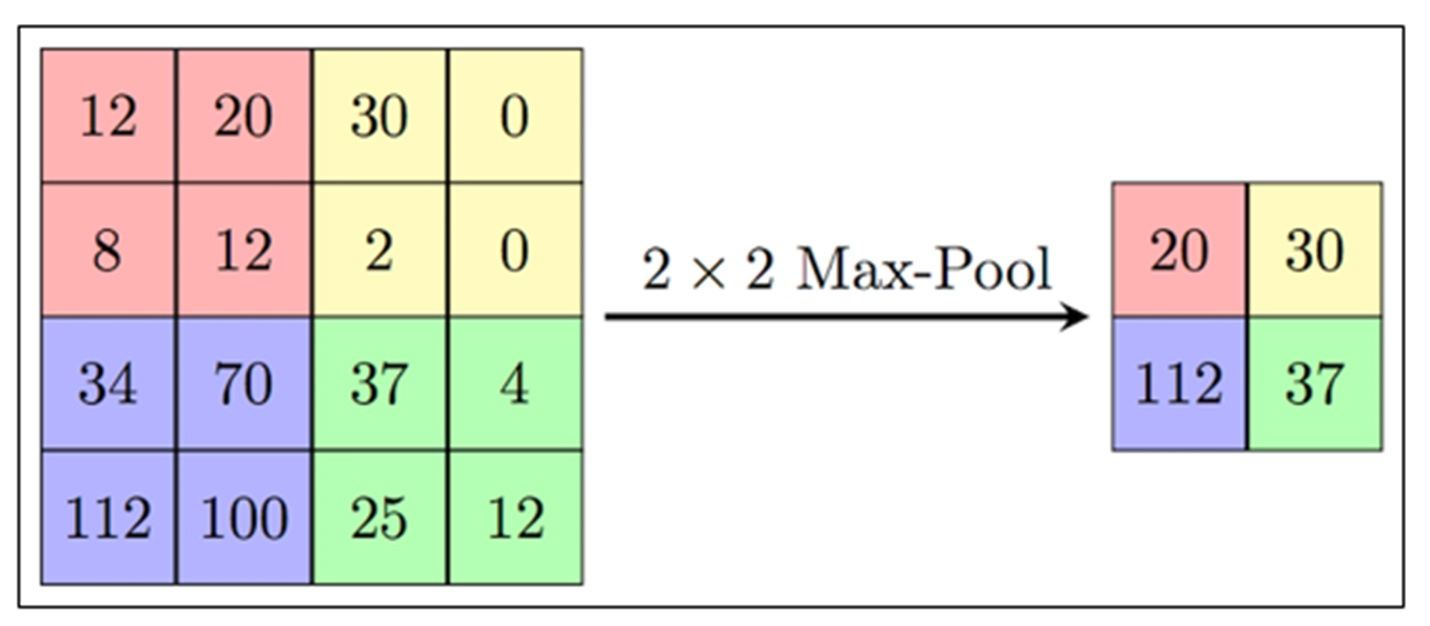
\includegraphics[width=0.7\linewidth]{images/maxpooling}
	\caption{Операция макспуллинга}
	\label{fig:maxpooling}
\end{figure}
Как правило, каждая карта этого слоя имеет размерность 2x2, что позволяет уменьшить изображение в два раза. Благодаря уменьшению размера увеличивается скорость вычислений, упрощается поиск признаков более высокого уровня на следующих сверточных слоях, так как ненужные детали отбрасываются.

Полносвязный слой является последним в структуре сверточной нейронной сети и представляет собой слой обычного многослойного перцептрона. Его цель -- классификация при помощи нелинейной функции, улучшая качество распознавания. Выходной слой связан со всеми нейронами предыдущего слоя, количество нейронов которого обычно соответствует количеству распознаваемых классов. 

Сверточные нейронные сети обучаются при помощи алгоритма обратного распространения ошибки. Сначала выполняется прямое распространение от первого слоя к последнему, после чего на выходном слое вычисляется ошибка, передающаяся обратно. На каждом слое вычисляются градиенты обучаемых параметров,, используемые для обновления весов при помощи градиентного спуска в конце обратного распространения.
\section{Техническое задание}
\subsection{Основание для разработки}

Основанием для разработки является задание на выпускную квалификационную работу бакалавра "<Интеллектуальная система мониторинга и распознавания загрязнений водоемов">.

\subsection{Цель и назначение разработки}

Программная система предназначения для автоматического распознавания пятен нефтяных разливов на изображениях и их визуального выделения.

Пользователи должны иметь возможность загружать собственные изображения для анализа системой. Также должен быть реализован функционал сохранения полученных результатов программного анализа .

Задачами данной разработки являются:
\begin{itemize}
\item создание интеллектуальной системы распознавания на основе технологий нейронных сетей;
\item обучение созданной интеллектуальной системы для распознавания пятен нефтяных разливов;
\item разработка функционала для тестирования точности анализа полученной системы;
\item реализация настольного приложения с графическим интерфейсом для взаимодействия пользователей с системой.
\end{itemize}

\subsection{Требования пользователя к программной системе}

\subsubsection{Требования к данным программной системы}

Для обучения нейронной сети и анализа изображений на предмет наличия пятен разливов нефти программной системе требуется датасет, состоящий из изображений в формате JPEG, сохраненные в отдельной папке. Кроме того, для сохранения параметров обученной модели нейронной сети используются файлы формата .pth, содержащие веса и смещения модели. Для анализа изображений и тестирования нейронной сети также требуются файлы в формате .pth, содержащие параметры, предварительно полученные после обучения нейронной сети.

\subsubsection{Функциональные требования к программной системе}

Разработанная программа должна реализовывать следующие функциональные возможности:

\begin{itemize}
	\item обучение нейронной сети: после выбора директории с изображениями, директории сохранения полученных параметров и параметров обучения, программа запускает обучение нейронной сети и, по его завершении, сохраняет полученный набор параметров в указанную пользователем директорию;
	\item тестирование нейронной сети: после загрузки тестового изображения и предварительно сохраненного файла параметров нейронной сети, программа должна обрабатывать полученное изображение при помощи модели сети, выводить результат анализа в виде бинарного изображения, идеальный ожидаемый результат, полученный с помощью простого алгоритма обработки и метрики, оценивающие эффективность работы нейронной сети;
	\item распознавание нефтяных пятен: программа должна распознавать пятна разливов нефти на фотографиях при помощи предоставленных пользователем параметров на загруженном изображении;
	\item сохранение результатов: пользователь должен иметь возможность сохранения проанализированных изображений на жесткий диск.	
\end{itemize}

На рисунке~\ref{fig:usecase} предоставлены функциональные требования к системе, представленные в виде диаграммы прецедентов\cite{fowler_uml}.

\begin{figure}[H]
	\centering
	\includegraphics[width=0.7\linewidth]{"images/сценарии использования"}
	\caption{Диаграмма прецедентов}
	\label{fig:usecase}
\end{figure}

\paragraph{Сценарий использования "<Обучение нейронной сети">}

Заинтересованные лица и их требования: пользователь желает обучить модель нейронной сети для распознавания нефтяных пятен на поверхности водоемов.

Предусловие: программа запущена, выбран режим "<Обучение">.

Постусловие: программа сохраняет файл, содержащий параметры весов нейронной сети.

Основной успешный сценарий:

\begin{enumerate}
	\item Пользователь нажимает на кнопку "<Выбрать папку">	.
	\item Программа открывает диалоговое окно выбора папки.
	\item Пользователь выбирает папку, содержащую изображения для обучения нейронной сети.
	\item Программа отображает путь до выбранной папки в специальном поле.
	\item Пользователь нажимает на кнопку "<Выбрать путь сохранения">.
	\item Программа открывает диалоговое окно выбора папки сохранения.
	\item Пользователь выбирает директорию, в которой будет сохранен файл, содержащий параметры нейронной сети.
	\item Программа отображает путь до выбранной директории сохранения в специальном поле.
	\item Пользователь выбирает количество изображений, обрабатываемых нейронной сетью одновременно (размер батча).
	\item Пользователь указывает количество эпох обучения.
	\item Пользователь нажимает на кнопку "<Обучить нейросеть">.
	\item Программа начинает процесс обучения нейронной сети на полученных изображениях, используя заданные параметры.
	\item Программа отображает прогресс процесса обучения пользователю.
	\item Программа сохраняет полученный файл, содержащий параметры нейронной сети в папку, указанную пользователем, после завершения процесса обучения.
\end{enumerate}

\paragraph{Сценарий использования "<Тестирование нейронной сети">}

Заинтересованные лица и их требования: пользователь желает протестировать работу предварительно обученную нейронную сеть и узнать качество сегментации.

Предусловие: программа запущена, выбран режим "<Тестирование">, имеется файл с настройками нейронной сети.

Постусловие: программа отображает метрики качества сегментации, а также сравнение ожидаемых и полученных результатов.

Основной успешный сценарий:

\begin{enumerate}
	\item Пользователь нажимает на кнопку "<Выбрать изображение">.
	\item Программа открывает диалоговое окно выбора изображения, используемого для тестирования нейронной сети.
	\item Пользователь выбирает изображение.
	\item Программа отображает путь до выбранного изображения в специальном поле.
	\item Пользователь нажимает на кнопку "<Выбрать настройки">.
	\item Программа открывает диалоговое окно выбора файла настроек нейронной сети.
	\item Пользователь выбирает файл настроек нейронной сети.
	\item Программа отображает путь до выбранного файла настроек в специальном поле.
	\item Пользователь нажимает на кнопку "<Запустить тестирование">.
	\item Программа выполняет предварительную обработку изображения.
	\item Программа создает ожидаемую маску на основании загруженного изображения при помощи порогового алгоритма.
	\item Программа обрабатывает обработанное изображение, используя нейронную сеть с загруженными параметрами.
	\item Программа рассчитывает метрики качества сегментации изображения.
	\item Программа отображает ожидаемую и полученную нейронной сетью маски классов, а также метрики качества сегментации.
\end{enumerate}

\paragraph{Сценарий использования "<Анализ изображения">}

Заинтересованные лица и их требования: пользователь желает проанализировать изображение на наличие нефтяного разлива.

Предусловие: программа запущена, выбран режим "<Анализ изображения">, имеется файл с настройками нейронной сети.

Постусловие: программа отображает результаты анализа изображения.

Основной успешный сценарий:

\begin{enumerate}
	\item Пользователь нажимает на кнопку "<Выбрать изображение">.
	\item Программа открывает диалоговое окно выбора анализируемого изображения.
	\item Пользователь выбирает необходимое изображение.
	\item Программа отображает путь до выбранного изображения в специальном поле и выводит его в главное окно.
	\item Пользователь нажимает на кнопку "<Выбрать модель">.
	\item Программа открывает диалоговое окно выбора файла с настройками модели.
	\item Пользователь выбирает файл настроек нейронной сети.
	\item Программа отображает путь до выбранного файла в специальном поле.
	\item Пользователь нажимает на кнопку "<Анализировать">.
	\item Программа выполняет предварительную обработку изображения.
	\item Программа анализирует обработанное изображение на предмет наличия пятен нефтяных разливов с помощью нейронной сети.
	\item Программа отображает результат анализа на исходной версии изображения, загруженной пользователем в главном окне программы.
\end{enumerate}

\paragraph{Сценарий использования "<Сохранение результата анализа">}

Заинтересованные лица и их требования: пользователь желает сохранить результат анализа изображения нейронной сетью.

Предусловие: программа запущена, выбран режим "<Анализ изображения">, изображение предварительно загружено и проанализированно.

Постусловие: программа сохраняет результат обработки в виде изображения на жесткий диск.

Основной успешный сценарий:

\begin{enumerate}
	\item Пользователь нажимает на кнопку "<Сохранить результат">.
	\item Программа открывает диалоговое окно выбора папки для сохранения результата анализа.
	\item Пользователь выбирает необходимую папку.
	\item Программа сохраняет результат анализа в указанную папку в виде изображения.
	\item Программа уведомляет пользователя об успешном сохранении изображения.
\end{enumerate}

\subsubsection{Требования пользователя к интерфейсу приложения}

Приложение должно иметь следующие экраны:

\begin{enumerate}
	\item Экран "<Анализ изображения">. Основной экран, реализующий функционал распознавания пятен нефти на изображениях поверхности водоемов, где реализована возможность загрузки изображения для поиска нефтяных пятен, просмотр результата работы нейронной сети и его сохранения на жесткий диск.
	\item Экран "<Обучение">. Экран, позволяющий обучать нейронную сеть искать пятна разливов нефти на изображениях. Должен содержать возможность выбора папки, содержащей датасет для обучения, и директории сохранения файла, содержащего настройки параметров нейронной сети, полученные во время ее обучения.
	\item Экран "<Тестирование">. Экран для тестирования обученной модели, позволяющий выбрать файл настроек нейронной сети, тестовое изображение, а также отображающий исходное изображение, ожидаемый результат и фактический результат обработки тестового изображения нейронной сетью.
\end{enumerate}

\subsection{Нефункциональные требования к программной системе}

\subsubsection{Требования к надежности}

Программная система должна обеспечивать стабильную работу в различных условиях эксплуатации. В процессе работы приложения могут возникнуть следующие аварийные ситуации:
\begin{itemize}
	\item отсутствие файлов изображений в папке, выбранной как директория хранения датапака;
	\item попытка загрузить в программу поврежденное изображение;
	\item ошибки загрузки или сохранения файлов настроек моделей или изображений из-за проблем с файловой системой;
	\item ошибки в работе программы из-за загрузки пользователем файлов некорректных форматов.
\end{itemize} 

Для предотвращения аварийных ситуаций программа должна корректно обрабатывать исключения при работе с файлами, предоставляя пользователям информативные сообщения об ошибках. В случае проблем с отсутствием прав доступа к  директории сохранения файлов, полученных в результате работы программы, программа должна открывать диалоговое окно с выбором другой директории.

\subsubsection{Требования к аппаратному обеспечению}

Для корректной работы программного продукта требуется центральный процессор с количеством ядер от 6 и выше с частотой ядра от 2.4 ГГц. Размер необходимой оперативной памяти - 8 Гб и выше. Кроме того, для отрисовки графического интерфейса требуется видеокарта с объемом графической памяти 4 Гб и выше, монитор. Наконец, для управления программой необходимы клавиатура и мышь.

Для ускорения процесса обучения нейронной сети возможно использование вычислительных ресурсов графического адаптера NVIDIA с поддержкой технологии CUDA. 

\subsubsection{Требования к программному обеспечению}

Для запуска и работы программы требуется компьютер под управлением операционной системы Windows 10 или Windows 11. При использовании графических адаптеров NVIDIA с поддержкой технологии CUDA для ускорения обучения нейронной сети необходима последняя версия драйверов соответствующего адаптера, а также программы CUDA Toolkit и cuDNN.

\subsection{Требования к оформлению документации}

Требования к стадиям разработки программ и программной документации для вычислительных машин, комплексов и систем независимо от их назначения и области применения, этапам и содержанию работ устанавливаются ГОСТ 19.102–77. и ГОСТ 34.601-90. 

Программная документация должна включать в себя:

\begin{itemize}
	\item анализ предметной области;
	\item техническое задания;
	\item технический проект;
	\item рабочий проект.
\end{itemize}

\section{Технический проект}
\subsection{Общая характеристика организации решения задачи}

Необходимо спроектировать и разработать интеллектуальную систему распознавания пятен разливов нефти на поверхности водоемов.

Интеллектуальная система состоит из модели нейронной сети и приложения, отвечающего за взаимодействие пользователей с системой. В приложении необходимо иметь возможность взаимодействовать с нейронной сетью при помощи графического интерфейса пользователя. Под взаимодействием понимается загрузка изображений, содержащих пятна нефтяных разливов, возможность распознавания пятен при помощи модели нейронной сети, а также её обучение и тестирование.

\subsection{Обоснование выбора технологии проектирования}

Технологии, языки программирования и архитектурные решения, использованные для создания интеллектуальной системы, отвечают современным практикам разработки и позволяют достичь высокой производительности и отказоустойчивости программы.

\subsubsection{Язык программирования Python}

Для реализации программной системы был использован язык Python. Python -- язык программирования высокого уровня, обладающий высокой степенью гибкости и широко используемый как в научной отрасли, так и для коммерческой разработки. Особенно хорошо Python подходит для построения интеллектуальных систем и анализа изображений благодаря богатой системе внешних библиотек, позволяющих значительно упростить построение модели нейронной сети, подготовку данных, работу с изображениями, создание графического интерфейса пользователя. 
Интуитивный синтаксис языка позволяет снизить количество синтаксических ошибок, что в свою очередь значительно ускоряет разработку программных продуктов. Встроенная поддержка различных парадигм программирования позволяет удобно реализовывать модульную архитектуру приложения с использованием классов, функций и последовательного кода. Кроссплатформенность языка облегчает адаптацию системы для работы на различных операционных систем, что при желании позволит легко создать нативные версии приложений для таких операционных систем, как Linux и macOS.


\subsubsection{Описание библиотеки PyTorch}
	
Для разработки модели нейронной сети была выбрана библиотека PyTorch. PyTorch является открытой библиотекой, содержащей широкий	набор инструментов для машинного обучения. Данная библиотека активно применяется в разнообразных научных исследованиях, использующих модели нейронных сетей. PyTorch зарекомендовала себя благодаря гибкости, лаконичному синтаксису и обширным возможностям построения и обучения нейронных сетей. 

Для определения структуры вычислений PyTorch использует динамический вычислительный граф, что означает построение графа операций непосредственно в процессе выполнения программы вместо предварительного определения его структуры. Данный подход значительно упрощает модификацию и отладку архитектуры модели нейронной сети, позволяет удобно реализовывать операции обучения, тестирования и анализа при помощи полученной модели нейронной сети. 

\subsubsection{Описание библиотеки OpenCV}

OpenCV -- одна из наиболее часто применяемых библиотек в области компьютерного зрения и обработки изображений. Она позволяет реализовать значительное количество операций для работы с изображениями и видео, таких как фильтрация, преобразования, геометрические операции. Высокая производительность позволяет эффективно читать, изменять размеры и форматы изображений, создавать их маски, визуализировать результаты работы интеллектуальной системы. 

\subsubsection{Описание фреймворка PyQt6}

PyQt6 является набором расширений кросплатформенного графического фреймворка Qt 6 версии для языка Python. PyQt6 позволяет создавать графические интерфейсы пользователя различной сложности -- от простых оконных приложений до многооконных систем с развитой логикой взаимодействий. 

Одним из ключевых преимуществ PyQt6 является большое число готовых элементов графического интерфейса, таких как кнопки, выпадающие списки, таблицы, позволяющих строить полноценный интуитивный пользовательский интерфейс. Графический интерфейс PyQt можно разрабатывать как вручную в коде, так и при помощи визуального редактора Qt Designer, возвращающего пользователю готовый Python-код для графического интерфейса. Кроссплатформенность PyQt6 позволяет запускать приложения, разработанные для операционной системы Windows на компьютерах с Linux и macOS не требуя значительных изменений, что позволяет без особых усилий создавать мультиплатформенные версии приложений.

\subsubsection{Описание библиотеки NumPy}

Библиотека NumPy предназначена для работы с многомерными массивами и матрицами, а также позволяет проводить сложные математические вычисления с высокой скоростью. NumPy предлагает большое количество функций для работы с массивами, таких как арифметические и логические операции, линейная алгебра. 

NumPy позволяет преобразовывать изображения и их маски в числовые массивы для дальнейшей обработки, а также объединять и нормализовать эти маски. Компактный синтаксис и высокая производительность делают его подходящим для практически любых проектов, связанных с обработкой данных. 

\subsection{Архитектура программной системы}

На рисунке~\ref{fig:structure} в виде UML-диаграммы представлена архитектура программной системы.  

\begin{figure}[h]
	\centering
	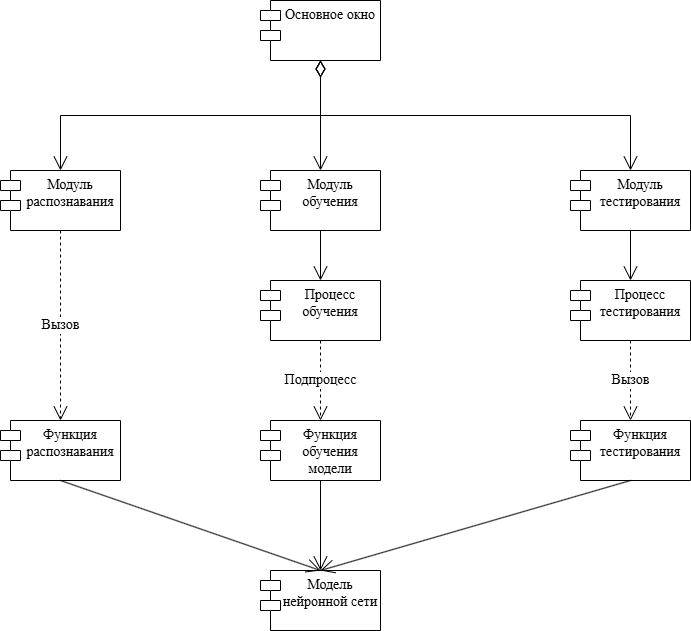
\includegraphics[width=0.85\linewidth]{images/компоненты}
	\caption{Архитектура системы}
	\label{fig:structure}
\end{figure}

Интеллектуальная система состоит из следующих компонентов:
\begin{enumerate}
	\item Основное окно. Основное окно отвечает за вызов главного окна программной системы и инициализацию трех режимов работы программы и переключение между ними.
	\item Модуль распознавания. Данный модуль вызывает окно для распознавания изображения, позволяющее выбрать изображение и параметры модели для анализа нейронной сетью, запускает процесс распознавания и отображает результат.
	\item Функция распознавания. Использует модель нейронной сети и ее параметры для анализа полученного изображения, возвращая результат работы и сохраняя его в виде файла.
	\item Модуль обучения. Вызывает окно, позволяющее выбрать директорию, содержащую изображения для обучения нейронной сети, и указать директорию для сохранения файла параметров обученной нейронной сети. Кроме того, данный модуль запускает процесс, отвечающий за обучение нейронной сети и отображение прогресса завершения обучения. 
	\item Функция обучения модели. Компонент загружает изображения для обучения, преобразует их в требуемый для обучения нейронной сети вид и обучает модель, сохраняя полученный в результате файл параметров.
	\item Модуль тестирования. Вызывает окно, позволяющее выбрать параметры модели, тестовое изображение и запускает процесс, отвечающий за тестирование модели нейронной сети с сохраненными параметрами и возвращает результаты тестирования. Также отображает полученные метрики и результаты.
	\item Функция тестирования. Выполняет оценку точности модели нейронной сети с параметрами, загруженными из предварительно сохраненного файла. Сравнивает результат анализа изображения нейронной сетью и ожидаемый результат, полученный при помощи пороговой фильтрации.
	\item Модель нейронной сети. Хранит в себе структуру используемой в системе нейронной сети. 
\end{enumerate}

\subsection{Выбор структуры нейронной сети}

Для распознавания нефтяных пятен на изображениях поверхностей водоемов была спроектирована и разработана модель сверточной нейронной сети. Сверточные нейронные сети -- однонаправленные модели, разработанные для распознавания образов на изображениях. В данной работе была реализована нейронная сеть типа U-Net, адаптированная под особенности предметной области. 

Архитектура U-Net была представлена в 2015 году группой исследователей из Университета Фрайбугра. Данная архитектура получила широкое распространение благодаря способности выделять объекты различной формы и масштаба с высокой точностью даже на маленьких обучающих выборках. Основной особенностью U-Net является симметричная структура: левая часть сети, или энкодер, выполняет последовательное сжатие входного изображения, а правая, или декодер -- восстановление пространственного разрешения до исходного размера.

\begin{figure}[h]
	\centering
	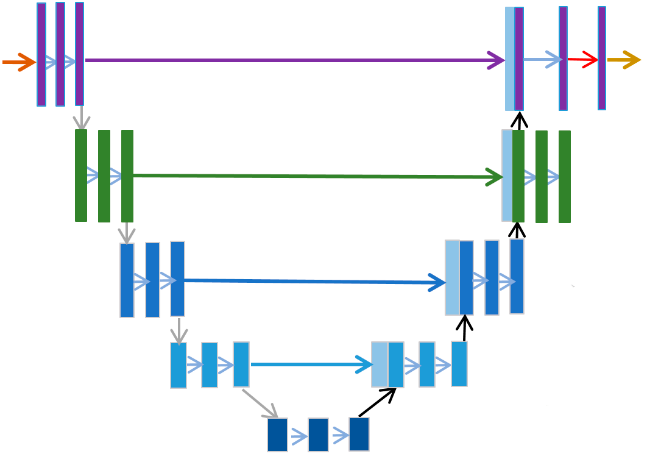
\includegraphics[width=0.85\linewidth]{images/unet}
	\caption{Архитектура сети U-Net}
	\label{fig:unet}
\end{figure}

Ключевым элементом U-Net являются прямые соединения между соответствующими уровнями энкодера и декодера, позволяющие использовать признаки, извлеченные на ранних этапах обработки, передавая их на этапы восстановления изображения, что предотвращает потерю пространственной информации. Данные особенности позволяют с легкостью адаптировать U-Net для использования в различных областях, например медицинская диагностика, спутниковый мониториг, обработка изображений, полученных с беспилотных летательных аппаратов.

\subsection{Проектирование пользовательского интерфейса}

На основании требований к пользовательскому интерфейсу, представленных в пункте 2.3.3, был разработан графический интерфейс программной системы. 

На рисунке~\ref{fig:uianalysis} представлен макет интерфейса окна "<Анализ изображения">. Макет содержит следующие элементы:

\begin{enumerate}
	\item Кнопка переключения режимов окна.
	\item Поле, содержащее путь до анализируемого изображения.
	\item Кнопка выбора изображения для анализа.
	\item Поле, содержащее путь до выбранного файла параметров нейронной сети.
	\item Кнопка выбора файла параметров нейронной сети.
	\item Поле для отображения загруженного изображения и результатов анализа.
	\item Кнопка для запуска распознавания нефтяных пятен. 
	\item Кнопка для сохранения результатов анализа нейронной сети.
\end{enumerate}

\begin{figure}[H]
	\centering
	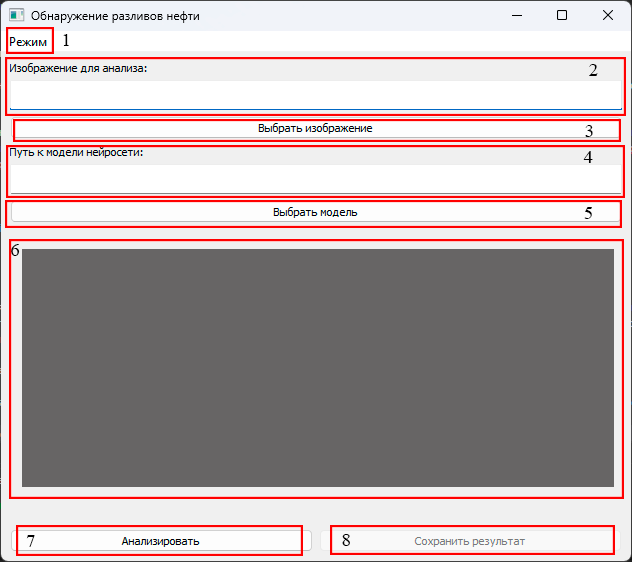
\includegraphics[width=1\linewidth]{images/ui_analysis}
	\caption{Макет интерфейса окна «Анализ изображения»}
	\label{fig:uianalysis}
\end{figure}

На рисунке~\ref{fig:uitrain} представлен макет интерфейса окна "<Обучение">. Макет содержит следующие элементы:

\begin{enumerate}
	\item Кнопка переключения режимов окна.
	\item Поле, содержащее путь до выбранной папки с изображениями для обучения нейронной сети.
	\item Кнопка выбора папки с изображениями для обучения нейронной сети.
	\item Поле, содержащее путь до папки, в которую необходимо сохранить параметры модели.
	\item Кнопка для выбора папки, в которую необходимо сохранить параметры модели.
	\item Окно для вывода прогресса обучения нейронной сети.
	\item Кнопка для запуска процесса обучения нейронной системы.
\end{enumerate}

\begin{figure}[H]
	\centering
	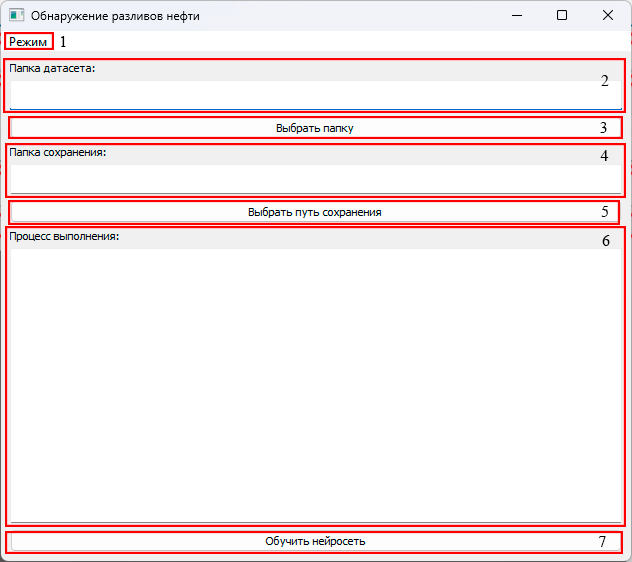
\includegraphics[width=1\linewidth]{images/ui_train}
	\caption{Макет интерфейса окна «Обучение»}
	\label{fig:uitrain}
\end{figure}

На рисунке~\ref{fig:uitest} представлен макет интерфейса окна "<Тестирование">. Макет содержит следующие элементы:

\begin{enumerate}
	\item Кнопка переключения режимов окна.
	\item Поле, содержащее путь до тестового изображения.
	\item Кнопка выбора изображения для тестирования нейронной сети.
	\item Поле, содержащее путь до выбранного файла параметров нейронной сети.
	\item Кнопка выбора файла параметров нейронной сети.
	\item Поле вывода метрик тестирования нейронной сети.
	\item Поле для отображения исходного изображения.
	\item Поле для отображения ожидаемого результата обработки.
	\item Поле для отображения фактического результата обработки изображения нейронной сети.
	\item Кнопка для запуска тестирования.
\end{enumerate}

\begin{figure}[H]
	\centering
	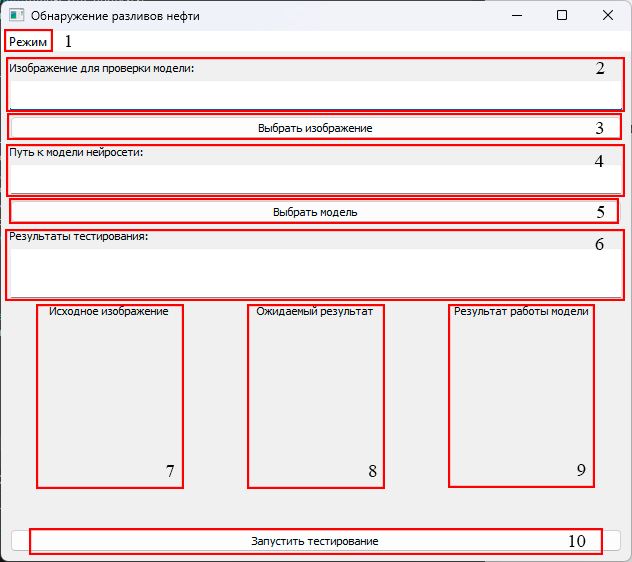
\includegraphics[width=1\linewidth]{images/ui_test}
	\caption{Макет интерфейса окна «Тестирование»}
	\label{fig:uitest}
\end{figure}

\newpage
\ifПрактика{}\else{
   \section{Рабочий проект}

\subsection{Спецификация компонентов и классов программы}

\subsubsection{Модуль main.py}

Модуль предоставляет графический интерфейс с меню для переключения между тремя режимами работы: анализ изображений, обучение и тестирование нейронной сети. 

Класс -- MainWindow.

Описание класса MainWindow.
Класс предназначен для управления главным окном приложения и переключения между режимами работы программы. Базовый класс -- QMainWindow, стандартный класс библиотеки PyQt5. Интерфейсы: панель меню, позволяющая переключать режимы работы программы; центральный виджет QStackedWidget, отображающий интерфейс активного режима работы. Константы: отсутствуют. Внутренние поля представлены в таблице~\ref{table:main_widgets}.

\begin{xltabular}{\textwidth}{|X|X|X|}
	\caption{Внутренние поля класса MainWindow\label{table:main_widgets}} \\
	\hline 
	\centrow Внутреннее поле & 
	\centrow Тип & 
	\centrow Описание \\ 
	\hline 
	\endfirsthead
	
	\caption*{Продолжение таблицы \ref{table:main_widgets}} \\
	\hline 
	\centrow Внутреннее поле & 
	\centrow Тип & 
	\centrow Описание \\ 
	\hline 
	\endhead
	
	stack & QStackedWidget & Содержит три виджета графического интерфейса для каждого режима работы программы \\ \hline
	analysis\_widget & ImageAnalysisWidget & Виджет, содержащий графический интерфейс режима анализа изображений \\ \hline
	training\_widget & TrainingWidget & Виджет, содержащий графический интерфейс режима обучения нейронной сети \\ \hline
	testing\_widget & TestingWidget & Виджет, содержащий графический интерфейс режима тестирования нейронной сети \\ \hline
\end{xltabular}
Методы класса представлены в таблице~\ref{table:main_method}.
\renewcommand{\arraystretch}{0.8} % уменьшение расстояний до сетки таблицы
\begin{xltabular}{\textwidth}{|>{\hsize=0.7\hsize\raggedright\arraybackslash}X|
		>{\hsize=1.0\hsize\setlength{\baselineskip}{0.7\baselineskip}}X|
		>{\hsize=1.0\hsize}X|
		>{\hsize=1.3\hsize}X|}
	\caption{Методы класса MainWindow\label{table:main_method}}\\
	\hline 
	\centrow \setlength{\baselineskip}{0.7\baselineskip} Название метода & 
	\centrow Параметры метода &
	\centrow Возвращаемое значение & 
	\centrow Назначение метода \\ 
	\hline 
	\endfirsthead
	
	\caption*{Продолжение таблицы \ref{table:main_method}}\\
	\hline 
	\centrow Название метода & 
	\centrow Параметры метода &
	\centrow Возвращаемое значение & 
	\centrow Назначение метода \\ 
	\hline 
	\endhead
	
	\_\_init\_\_ & Не имеет & Не имеет  & Инициализирует главное окно программы, задает его параметры, заголовок, панель меню с действиями для переключения режимов \\ \hline 
	switch\_mode & index --  идентификатор  активного режима окна& Не имеет& Переключает графический интерфейс в соответствии с выбранным режимом работы \\ \hline
	
\end{xltabular}
\renewcommand{\arraystretch}{1.0} % восстановление сетки
\vspace{-\baselineskip}

\subsubsection{Модуль model.py}

Модуль определяет структуру нейронной сети UNet, используемой для обнаружения разливов нефти.

Класс -- UNet.

Описание класса UNet.
Класс реализует модель UNet для сегментации и распознавания пятен нефтяных разливов на поверхности водоемов. Базовый класс --  nn.Module, стандартный класс библиотеки PyTorch. Интерфейсы: общедоступные методы \_\_init\_\_ и forward. Константы отсутствуют. Внутренние поля представлены в таблице~\ref{table:network_components}.
\begin{xltabular}{\textwidth}{|X|X|X|}
	\caption{Внутренние поля класса UNet \label{table:network_components}} \\
	\hline 
	\centrow Внутреннее поле & 
	\centrow Тип & 
	\centrow Описание \\ 
	\hline 
	\endfirsthead
	
	\caption*{Продолжение таблицы \ref{table:network_components}} \\
	\hline 
	\centrow Внутреннее поле & 
	\centrow Тип & 
	\centrow Описание \\ 
	\hline 
	\endhead
	
	enc1 & nn.Sequential & Первый блок энкодера \\ \hline
	enc2 & nn.Sequential & Второй блок энкодера \\ \hline
	pool & nn.MaxPool2d & Слой максимального пуллинга, уменьшающий разрешение \\ \hline
	bottleneck & nn.Sequential & Блок узкого места \\ \hline
	upconv2 & nn.ConvTranspose2d & Второй слой повышения разрешения \\ \hline
	dec2 & nn.Sequential & Второй блок декодера \\ \hline
	upconv1 & nn.ConvTranspose2d & Первый слой повышения разрешения \\ \hline
	dec1 & nn.Sequential & Первый блок декодера \\ \hline
	final\_conv & nn.Conv2d & Финальный сверточный слой, создающий выходную маску признаков \\ \hline
\end{xltabular}
Методы класса представлены в таблице~\ref{table:model_method}.
\renewcommand{\arraystretch}{0.8} % уменьшение расстояний до сетки таблицы
\begin{xltabular}{\textwidth}{|>{\hsize=0.7\hsize\raggedright\arraybackslash}X|
		>{\hsize=1.0\hsize\setlength{\baselineskip}{0.7\baselineskip}}X|
		>{\hsize=1.0\hsize}X|
		>{\hsize=1.3\hsize}X|}
	\caption{Методы класса UNet\label{table:model_method}}\\
	\hline 
	\centrow Название метода & 
	\centrow Параметры метода & 
	\centrow Возвращаемое значение &
	\centrow Назначение метода \\ 
	\hline 
	\endfirsthead
	
	\caption*{Продолжение таблицы \ref{table:model_method}}\\
	\hline 
	\centrow Название метода & 
	\centrow Параметры метода & 
	\centrow Возвращаемое значение &
	\centrow Назначение метода \\ 
	\hline 
	\endhead
	
	\_\_init\_\_ & \parbox[t]{\linewidth}{in\_channels -- количество входных каналов; \\ out\_channels -- количество выходных каналов}  & Не имеет & Инициализирует архитектуру UNet \\ \hline 
	forward & x -- входной тензор & torch.Tensor -- выходная маска признаков & Выполняет прямой проход через нейронную сеть, возвращая итог сегментации \\ \hline
	conv\_block & \parbox[t]{\linewidth}{ in\_c --  входные каналы; \\ out\_c -- выходные каналы}& nn.Sequential -- контейнер сверточного блока & Определяет сверточный блок с двумя сверточными слоями и функциями активации\\ \hline
	
\end{xltabular}
\renewcommand{\arraystretch}{1.0} % восстановление сетки
\vspace{-\baselineskip}

\subsubsection{Модуль test.py}

Модуль содержит функции для оценки обученной модели UNet на одном изображении.  Не содержит классов. Методы модуля:
\begin{enumerate}
	\item dice\_coefficient. Вычисляет коэффициент Dice для предсказанной маски. Входные данные:
	\begin{itemize}
		\item pred (тип torch.Tensor) -- предсказанная маска;
		\item target (тип torch.Tensor ) -- целевая маска;
		\item smooth (тип float,  значение по умолчанию -- 1e$^{-6} $) -- стабилизирующая константа для избежания деления на ноль.
	\end{itemize}
	Возвращаемые данные -- коэффициент Dice в виде float-числа.
	\item iou\_score. Вычисляет пересечение по объединению (коэффициент IoU) для предсказанной маски. Входные данные:
	\begin{itemize}
		\item pred (тип torch.Tensor) -- предсказанная маска;
		\item target (тип torch.Tensor ) -- целевая маска;
		\item smooth (тип float,  значение по умолчанию -- 1e$^{-6} $) -- стабилизирующая константа для избежания деления на ноль.
	\end{itemize}
	Возвращаемые данные -- коэффициент пересечения по объединению в виде float-числа.
	\item load\_image. Загружает изображение и выполняет предобработку для дальнейшего анализа нейронной сетью. Входные данные:
	\begin{itemize}
		\item path (тип str) -- путь к загружаемому изображению;
		\item size (тип tuple) -- целевой размер изображения для дальнейшей обработки нейронной сетью.
	\end{itemize}
	Возвращаемые данные: нормализованный массив изображения типа np.ndarray.
	\item run\_evaluation. Выполняет оценку точности обученной модели нейронной сети и возвращает результаты обработки и метрики. Входные данные:
	\begin{itemize}
		\item image\_path (тип str) -- путь к анализируемому изображению;
		\item weights (тип str) -- путь к оцениваемым весам модели;
		\item threshold (тип float, значение по умолчанию = 0,3) -- порог для бинаризации масок
	\end{itemize}
	Возвращаемые данные -- значения коэффициентов Dice и IoU, исходное изображение, ожидаемую маску, полученную при помощи пороговой бинаризации и предсказанную сетью маску в виде словаря dict.
\end{enumerate}

\subsubsection{Модуль train.py}

Модуль управляет загрузкой датасета и обучением нейронной сети.

Классы: dataset и Trainer.

Описание класса dataset.
Класс загружает и предобрабатывает изображения и создает псевдомаски на основании порога для обучения нейронной сети. Базовый класс -- Dataset, стандартный класс библиотеки PyTorch. Интерфейсы -- общедоступные методы \_\_init\_\_, \_\_len\_\_, \_\_getitem\_\_, общедоступные атрибуты image\_dir, images. Константы отсутствуют. Внутренние поля представлены в таблице~\ref{table:dataset_params}.
\begin{xltabular}{\textwidth}{|X|X|X|}
	\caption{Внутренние поля класса dataset \label{table:dataset_params}} \\
	\hline 
	\centrow Внутреннее поле & 
	\centrow Тип & 
	\centrow Описание \\ 
	\hline 
	\endfirsthead
	
	\caption*{Продолжение таблицы \ref{table:dataset_params}} \\
	\hline 
	\centrow Внутреннее поле & 
	\centrow Тип & 
	\centrow Описание \\ 
	\hline 
	\endhead
	
	image\_dir & str & Папка, содержащая датасет \\ \hline
	images & list & Список имен файлов изображений для обучения \\ \hline
	threshold & float & Порог для создания обучающих масок \\ \hline
\end{xltabular}
Методы класса представлены в таблице~\ref{table:dataset_method}. 
\renewcommand{\arraystretch}{0.8} % уменьшение расстояний до сетки таблицы
\begin{xltabular}{\textwidth}{|>{\hsize=0.7\hsize\raggedright\arraybackslash}X|
		>{\hsize=1.0\hsize\setlength{\baselineskip}{0.7\baselineskip}}X|
		>{\hsize=1.0\hsize}X|
		>{\hsize=1.3\hsize}X|}
	\caption{Методы класса dataset\label{table:dataset_method}}\\
	\hline 
	\centrow Название метода & 
	\centrow Параметры метода & 
	\centrow Возвращаемое значение &
	\centrow Назначение метода \\ 
	\hline 
	\endfirsthead
	
	\caption*{Продолжение таблицы \ref{table:dataset_method}}\\
	\hline 
	\centrow Название метода & 
	\centrow Параметры метода & 
	\centrow Возвращаемое значение &
	\centrow Назначение метода \\ 
	\hline 
	\endhead
	
	\_\_init\_\_ & \parbox[t]{\linewidth}{image\_dir -- путь к папке с датасетом; \\ threshold -- порог для создания обучающих масок} & Не имеет & Инициализирует датасет, проверяя директорию и загружая имена файлов изображений \\ \hline 
	\_\_len\_\_ & Не имеет & Количество изображений в датасете & Определяет количество изображений в датасете \\ \hline
	\_\_getitem\_\_ & idx -- порядковый номер обрабатываемого изображения & тензор изображения и маски & Загружает, предобрабатывает и создает обучающую маску для изображений датасета \\ \hline
	
\end{xltabular}
\renewcommand{\arraystretch}{1.0} % восстановление сетки
\vspace{-\baselineskip}

Описание класса Trainer.
Класс управляет обучением модели нейронной сети и отправляет сигналы о состоянии процесса обучения для обновления графического интерфейса. Базовый класс -- QObject, стандартный класс библиотеки PyQt5. Интерфейсы -- сигналы о состоянии процесса обучения, общедоступный метод \_\_init\_\_. Константы отсутствуют. Внутренние поля представлены в таблице~\ref{table:training_signals}.
\begin{xltabular}{\textwidth}{|X|X|X|}
	\caption{Внутренние поля класса Trainer\label{table:training_signals}}\\
	\hline 
	\centrow Внутреннее поле & 
	\centrow Тип & 
	\centrow Описание \\ 
	\hline 
	\endfirsthead
	
	\caption*{Продолжение таблицы \ref{table:training_signals}}\\
	\hline 
	\centrow Внутреннее поле & 
	\centrow Тип & 
	\centrow Описание \\ 
	\hline 
	\endhead
	
	\hline 
	\endfoot
	
	epoch\_start\_signal & pyqtSignal[int, int] & сигнал начала эпохи, содержащий её номер и общее количество эпох \\ \hline
	epoch\_complete\_signal & pyqtSignal[[int, float, float, float, float] & сигнал завершения эпохи, содержащий её номер и средние значения потерь при обучении, потерь на тестовой выборке, метрик Dice и IoU \\ \hline
	batch\_progress\_signal & pyqtSignal[int, int, float] & сигнал прогресса обработки батча, содержащий его номер, потерю, общее число батчей \\ \hline
	training\_complete\_signal & pyqtSignal[str] & сигнал завершения обучения \\ \hline
	image\_dir & str & Путь к папке с датасетом \\ \hline
	save\_path & str & Путь для сохранения весов модели \\ \hline
	batch\_size & int & Размер батча для обучения \\ \hline
	epochs & int & Количество эпох обучения \\ \hline
	lr & float & Скорость обучения \\ \hline
	threshold & float & Порог для создания обучающих и тестовых масок \\ \hline
\end{xltabular}
Методы класса представлены в таблице~\ref{table:Trainer_method}.
\renewcommand{\arraystretch}{0.8} % уменьшение расстояний до сетки таблицы
\begin{xltabular}{\textwidth}{|>{\hsize=0.7\hsize\raggedright\arraybackslash}X|
		>{\hsize=1.0\hsize\setlength{\baselineskip}{0.7\baselineskip}}X|
		>{\hsize=1.0\hsize}X|
		>{\hsize=1.3\hsize}X|}
	\caption{Методы класса Trainer\label{table:Trainer_method}}\\
	\hline 
	\centrow \setlength{\baselineskip}{0.7\baselineskip} Название метода & 
	\centrow Параметры метода & 
	\centrow Возвращаемое значение & 
	\centrow Назначение метода \\ 
	\hline 
	\endfirsthead
	
	\caption*{Продолжение таблицы \ref{table:Trainer_method}}\\
	\hline 
	\centrow Название метода & 
	\centrow Параметры метода & 
	\centrow Возвращаемое значение &
	\centrow Назначение метода \\ 
	\hline 
	\endhead
	
	\_\_init\_\_ & \parbox[t]{\linewidth}{image\_dir -- путь датасета; \\ save\_path -- путь сохранения весов; \\ batch\_size -- размер батча; \\ epochs -- количество эпох;\\  lr -- скорость обучения; \\ threshold -- порог для обучающих масок}  & Не имеет & Инициализирует процесс обучения с определенными параметрами \\ \hline 
	run & Не имеет & Не имеет & Обучает нейронную сеть, отправляя сигналы о прогрессе, и сохраняет параметры модели по завершении обучения \\ \hline
	
\end{xltabular}
\renewcommand{\arraystretch}{1.0} % восстановление сетки
\vspace{-\baselineskip}

В модуле train.py также реализован метод main(), предназначенная для получения аргументов обучения из графического интерфейса и запуска обучения при помощи Trainer. Метод не имеет входных и возвращаемых данных.

\subsubsection{Модуль detect.py}

Модуль используется для анализа изображений с использованием обученной модели нейронной сети, обнаруживая и выделяя пятна нефтяных разливов.  Не содержит классов. Методы модуля:
\begin{enumerate}
	\item load\_model. Загружает и инициализирует модель нейронной сети с указанными параметрами. Входные данные -- model\_path (тип str) -- путь к файлу параметров модели. Возвращаемые данные -- элемент класса Unet модуля model.py с загруженными из файла весами.
	\item analyze\_return. Метод обрабатывает изображение, используя нейронную сеть, создает бинарную маску разлива и возвращает исходное изображение с выделенными распознанными пятнами нефтяных разливов. Входные данные:
	\begin{itemize}
		\item image\_path (тип str) -- путь к анализируемому изображению;
		\item model\_path (тип str) -- путь к файлу параметров нейронной сети;
		\item threshold (тип float, значение по умолчанию -- 0,3) -- порог для бинаризации маски.
	\end{itemize}
	Возвращаемые данные -- изображение с выделенными распознанными нефтяными пятнами в формате np.ndarray.
\end{enumerate}

\subsubsection{Модуль analyze\_ui.py}

Модуль содержит графический интерфейс режима анализа изображений с использованием предварительно обученной модели нейронной сети.

Класс -- ImageAnalysisWidget. 

Описание класса ImageAnalysisWidget.
Класс содержит графический интерфейс, позволяющий выбрать анализируемое изображение, файл параметров нейронной сети, запустить процесс анализа и сохранить результат и отображающий этот результат. Базовый класс -- QWidget, стандартный класс библиотеки PyQt5. Интерфейсы -- поля для путей к изображению и модели, кнопки для выбора этих путей, начала анализа, сохранения результата, область отображения изображения. Константы отсутствуют. Внутренние поля класса представлены в таблице~\ref{table:image_analysis_elements}.
\begin{xltabular}{\textwidth}{|X|X|X|}
	\caption{Внутренние поля класса ImageAnalysisWidget\label{table:image_analysis_elements}}\\
	\hline 
	\centrow Внутреннее поле & 
	\centrow Тип & 
	\centrow Описание \\ 
	\hline 
	\endfirsthead
	
	\caption*{Продолжение таблицы \ref{table:image_analysis_elements}}\\
	\hline 
	\centrow Внутреннее поле & 
	\centrow Тип & 
	\centrow Описание \\ 
	\hline 
	\endhead
	
	\hline 
	\endfoot
	
	image\_path & str & путь к выбранному изображению \\ \hline
	model\_path & str & путь к выбранному файлу параметров нейронной сети \\ \hline
	result\_img & np.ndarray & проанализированное изображение с разметкой \\ \hline
	path\_label & QLabel & надпись "Изображение для анализа:" \\ \hline
	path\_field & QTextEdit & текстовое поле для отображения пути к изображению \\ \hline
	select\_button & QPushButton & кнопка для выбора изображения \\ \hline
	model\_label & QLabel & надпись "Путь к модели нейросети:" \\ \hline
	model\_path\_field & QTextEdit & текстовое поле для отображения пути к модели \\ \hline
	select\_model\_button & QPushButton & кнопка для выбора файла параметров \\ \hline
	image\_label & QLabel & поле для отображения изображения \\ \hline
	analyze\_button & QPushButton & кнопка для анализа изображения \\ \hline
	save\_button & QPushButton & кнопка для сохранения результата анализа \\ \hline
\end{xltabular}
Методы класса представлены в таблице~\ref{table:analyze_ui_method}.
\renewcommand{\arraystretch}{0.8} % уменьшение расстояний до сетки таблицы
\begin{xltabular}{\textwidth}{|>{\hsize=0.7\hsize\raggedright\arraybackslash}X|
		>{\hsize=1.0\hsize\setlength{\baselineskip}{0.7\baselineskip}}X|
		>{\hsize=1.0\hsize}X|
		>{\hsize=1.3\hsize}X|}
	\caption{Методы класса ImageAnalysisWidget\label{table:analyze_ui_method}}\\
	\hline 
	\centrow \setlength{\baselineskip}{0.7\baselineskip} Название метода & 
	\centrow Параметры метода & 
	\centrow Возвращаемое значение & 
	\centrow Назначение метода \\ 
	\hline 
	\endfirsthead
	
	\caption*{Продолжение таблицы \ref{table:analyze_ui_method}}\\
	\hline 
	\centrow Название метода & 
	\centrow Параметры метода & 
	\centrow Возвращаемое значение &
	\centrow Назначение метода \\ 
	\hline 
	\endhead
	
	\_\_init\_\_ & Не имеет & Не имеет  & Инициализирует графический интерфейс, включая его макет и элементы  \\ \hline 
	select\_image & Не имеет & Не имеет & Открывает диалоговое окно выбора изображения, отображает путь к нему и само изображение в интерфейсе \\ \hline
	select\_model & Не имеет & Не имеет & Открывает диалоговое окно выбора файла настроек модели и отображает путь к нему \\ \hline
	\parbox[t]{\linewidth}{analyze\_ \\ image} & Не имеет & Не имеет & Анализирует загруженное изображение при помощи нейронной сети и отображает результат распознавания \\ \hline
	save\_result & Не имеет & Не имеет & Открывает диалоговое окно выбора папки сохранения результата анализа изображения и сохраняет результат \\ \hline
	
\end{xltabular}
\renewcommand{\arraystretch}{1.0} % восстановление сетки
\vspace{-\baselineskip}

\subsubsection{Модуль train\_ui.py}

Модуль содержит графический интерфейс для настройки параметров и запуска процесса обучения модели нейронной сети.

Классы: TrainingThread, TrainingWidget.

Описание класса TrainingThread.
Данный класс выполняет процесс обучений нейронной сети в отдельном потоке для избежания блокировки и зависания графического интерфейса. Базовый класс -- QThread, стандартный класс библиотеки PyQt5. Интерфейсы -- сигналы для передачи прогресса обучения и обработки ошибок, функция, управляющая процессом обучения. Константы отсутствуют. Внутренние поля представлены в таблице~\ref{table:training_components}.
\begin{xltabular}{\textwidth}{|X|X|X|}
	\caption{Внутренние поля класса TrainingThread\label{table:training_components}}\\
	\hline 
	\centrow Внутреннее поле & 
	\centrow Тип & 
	\centrow Описание \\ 
	\hline 
	\endfirsthead
	
	\caption*{Продолжение таблицы \ref{table:training_components}}\\
	\hline 
	\centrow Внутреннее поле & 
	\centrow Тип & 
	\centrow Описание \\ 
	\hline 
	\endhead
	
	\hline 
	\endfoot
	
	trainer & Trainer & экземпляр класса Trainer из train.py для обучения нейронной сети \\ \hline
	error\_signal & pyqtSignal[str] & сигнал для передачи сообщений об ошибках в процессе обучения \\ \hline
\end{xltabular}
Методы класса представлены в таблице~\ref{table:TrainingThread_method}.
\renewcommand{\arraystretch}{0.8} % уменьшение расстояний до сетки таблицы
\begin{xltabular}{\textwidth}{|>{\hsize=0.7\hsize\raggedright\arraybackslash}X|
		>{\hsize=1.0\hsize\setlength{\baselineskip}{0.7\baselineskip}}X|
		>{\hsize=1.0\hsize}X|
		>{\hsize=1.3\hsize}X|}
	\caption{Методы класса TrainigThread\label{table:TrainingThread_method}}\\
	\hline 
	\centrow \setlength{\baselineskip}{0.7\baselineskip} Название метода & 
	\centrow Параметры метода & 
	\centrow Возвращаемое значение & 
	\centrow Назначение метода \\ 
	\hline 
	\endfirsthead
	
	\caption*{Продолжение таблицы \ref{table:TrainingThread_method}}\\
	\hline 
	\centrow Название метода & 
	\centrow Параметры метода & 
	\centrow Возвращаемое значение &
	\centrow Назначение метода \\ 
	\hline 
	\endhead
	
	\_\_init\_\_ & \parbox[t]{\linewidth}{dataset\_path -- путь к датасету; \\ model\_path -- путь к директории сохранения модели; \\ batch\_size -- размер батча; \\ epochs -- количество эпох обучения}  & Не имеет & Инициализирует поток обучения нейронной сети с экземпляром класса Trainer  \\ \hline 
	run & Не имеет & Не имеет & Выполняет обучение нейронной сети с обработкой ошибок \\ \hline
	
\end{xltabular}
\renewcommand{\arraystretch}{1.0} % восстановление сетки
\vspace{-\baselineskip}

Описание класса TrainingWidget.
Класс предоставляет графиеский интерфейс для выбора параметров обучения и отображения прогресса. Базовый класс -- QWidget, стандартный класс PyQt5. Интерфейсы -- поля ввода расположений датасета и сохранения результата, кнопки выбора путей, запуска обучения, шкала прогресса завершения обучения, текстовое поле для отображения сведений об обучении. Константы отсутствуют. Внутренние поля представлены в таблице~\ref{table:training_interface}.
\begin{xltabular}{\textwidth}{|X|X|X|}
	\caption{Внутренние поля класса TrainingWidget\label{table:training_interface}}\\
	\hline 
	\centrow Внутреннее поле & 
	\centrow Тип & 
	\centrow Описание \\ 
	\hline 
	\endfirsthead
	
	\caption*{Продолжение таблицы \ref{table:training_interface}}\\
	\hline 
	\centrow Внутреннее поле & 
	\centrow Тип & 
	\centrow Описание \\ 
	\hline 
	\endhead
	
	\hline 
	\endfoot
	
	dataset\_label & QLabel & надпись "<Папка датасета:>"\\ \hline
	dataset\_path\_field & QTextEdit & поле для отображения выбранной папки датасета \\ \hline
	select\_dataset\_button & QPushButton & кнопка для выбора папки датасета \\ \hline
	model\_label & QLabel & надпись "<Папка сохранения:>" \\ \hline
	model\_path\_field & QTextEdit & поле для отображения выбранной папки сохранения \\ \hline
	select\_model\_button & QPushButton & кнопка для выбора папки сохранения \\ \hline
	batch\_size\_label & QLabel & надпись "<Размер батча:>" \\ \hline
	batch\_size\_combo & QComboBox & выпадающий список для выбора размера батча \\ \hline
	epochs\_label & QLabel & надпись "Количество эпох:" \\ \hline
	epochs\_field & QLineEdit & поле для ввода количества эпох обучения \\ \hline
	progress\_label & QLabel & надпись "Прогресс эпохи:" \\ \hline
	progress\_bar & QProgressBar & шкала прогресса обучения нейронной сети \\ \hline
	log\_label & QLabel & надпись "Процесс выполнения:" \\ \hline
	output\_text & QTextEdit & поле для отображения сведений о процессе обучения \\ \hline
	train\_button & QPushButton & кнопка для запуска обучения \\ \hline
	thread & TrainingThread & поток для процесса обучения \\ \hline
\end{xltabular}
Методы класса представлены в таблице~\ref{table:TrainingWidget_method}.
\renewcommand{\arraystretch}{0.8} % уменьшение расстояний до сетки таблицы
\begin{xltabular}{\textwidth}{|>{\hsize=0.7\hsize\raggedright\arraybackslash}X|
		>{\hsize=1.0\hsize\setlength{\baselineskip}{0.7\baselineskip}}X|
		>{\hsize=1.0\hsize}X|
		>{\hsize=1.3\hsize}X|}
	\caption{Методы класса TrainigWidget\label{table:TrainingWidget_method}}\\
	\hline 
	\centrow \setlength{\baselineskip}{0.7\baselineskip} Название метода & 
	\centrow Параметры метода & 
	\centrow Возвращаемое значение &  
	\centrow Назначение метода \\ 
	\hline 
	\endfirsthead
	
	\caption*{Продолжение таблицы \ref{table:TrainingWidget_method}}\\
	\hline 
	\centrow Название метода & 
	\centrow Параметры метода & 
	\centrow Возвращаемое значение & 
	\centrow Назначение метода \\ 
	\hline 
	\endhead
	
	\_\_init\_\_ & Не имеет & Не имеет  & Инициализирует графический интерфейс, включая макет и элементы для настройки обучения и отображения прогресса  \\ \hline 
	\parbox[t]{\linewidth}{select\_dataset \\ \_folder} & Не имеет & Не имеет & Открывает диалоговое окно для выбора папки, содержащей датасет \\ \hline
	\parbox[t]{\linewidth}{select\_model\\ \_path} & Не имеет & Не имеет & Открывает диалоговое окно для выбора папки сохранения весов обученной нейронной сети \\ \hline
	run\_training & Не имеет & Не имеет & Проверяет корректность параметров обучения, заданных пользователем, отображает ошибки при наличии, создает поток обучения, подключает сигналы для обновления графического интерфейса \\ \hline
	\parbox[t]{\linewidth}{on\_epoch\_ \\ start} & \parbox[t]{\linewidth}{epoch -- номер текущей эпохи обучения; \\ total\_epochs -- общее количество эпох} & Не имеет & Обновляет отображаемый журнал обучения нейронной сети записью о начале эпохи и сбрасывает шкалу прогресса при начале новой эпохи обучения \\ \hline
	\parbox[t]{\linewidth}{on\_epoch\_ \\ complete} & \parbox[t]{\linewidth}{epoch -- номер завершенной эпохи; \\ avg\_loss -- среднее значение потери за эпоху обучения} & Не имеет & Обновляет отображаемый журнал информацией о завершении эпохи и заполняет шкалу прогресса по окончании эпохи обучения\\ \hline
	\parbox[t]{\linewidth}{on\_batch\_ \\ progress} & \parbox[t]{\linewidth}{batch -- номер текущего батча; \\ total\_batches -- общее количество батчей; \\ loss -- значение потери для текущего батча} & Не имеет & Обновляет шкалу прогресса в процессе обучения \\ \hline
	\parbox[t]{\linewidth}{append\_ \\ output} & text --  текст, добавляемый в журнал обучения& Не имеет & Добавляет текст в область отображения журнала \\ \hline
	show\_error & error\_message --  отображаемое сообщение об ошибке & Не имеет & Отображает диалоговое окно ошибки \\ \hline
	
\end{xltabular}
\renewcommand{\arraystretch}{1.0} % восстановление сетки
\vspace{-\baselineskip}

\subsubsection{Модуль test\_ui.py}

Модуль предоставляет графический интерфейс для тестирования модели нейронной сети.

Классы: TestingThread, TestingWidget.

Описание класса TestingThread.
Класс выполняет оценку модели в отдельном потоке, чтобы избежать зависаний графического интерфейса. Базовый класс -- QThread, стандартный класс PyQt5. Интерфейсы класса -- сигналы для обновления графического интерфейса. Константы отсутствуют. Внутренние поля представлены в таблице~\ref{table:testing_components}.
\begin{xltabular}{\textwidth}{|X|X|X|}
	\caption{Внутренние поля класса TestingThread\label{table:testing_components}}\\
	\hline 
	\centrow Внутреннее поле & 
	\centrow Тип & 
	\centrow Описание \\ 
	\hline 
	\endfirsthead
	
	\caption*{Продолжение таблицы \ref{table:testing_components}}\\
	\hline 
	\centrow Внутреннее поле & 
	\centrow Тип & 
	\centrow Описание \\ 
	\hline 
	\endhead
	
	\hline 
	\endfoot
	
	image\_path & str & путь к тестовому изображению \\ \hline
	model\_path & str & путь к файлу настроек модели нейронной сети \\ \hline
	output\_signal & pyqtSignal[str] & сигнал для сообщений о результатах тестирования \\ \hline
	results\_signal & pyqtSignal[dict] & сигнал для передачи результатов оценки \\ \hline
	error\_signal & pyqtSignal[str] & сигнал для сообщений об ошибках тестирования \\ \hline
\end{xltabular}
Методы класса представлены в таблице~\ref{table:TestingThread_method}.
\renewcommand{\arraystretch}{0.8} % уменьшение расстояний до сетки таблицы
\begin{xltabular}{\textwidth}{|>{\hsize=0.7\hsize\raggedright\arraybackslash}X|
		>{\hsize=1.0\hsize\setlength{\baselineskip}{0.7\baselineskip}}X|
		>{\hsize=1.0\hsize}X|
		>{\hsize=1.3\hsize}X|}
	\caption{Методы класса TestingThread\label{table:TestingThread_method}}\\
	\hline 
	\centrow \setlength{\baselineskip}{0.7\baselineskip} Название метода & 
	\centrow Параметры метода & 
	\centrow Возвращаемое значение &  
	\centrow Назначение метода \\ 
	\hline 
	\endfirsthead
	
	\caption*{Продолжение таблицы \ref{table:TestingThread_method}}\\
	\hline 
	\centrow Название метода & 
	\centrow Параметры метода & 
	\centrow Возвращаемое значение & 
	\centrow Назначение метода \\ 
	\hline 
	\endhead
	
	\_\_init\_\_ &  \parbox[t]{\linewidth}{image\_path -- путь к тестовому изображению; \\ model\_path -- путь к файлу параметров нейронной сети} & Не имеет  & Инициализирует поток, передавая в него пути к тестовому изображению и папке модели  \\ \hline 
	run & Не имеет & Не имеет & Выполняет оценку нейронной сети, отправляя результаты или ошибки через сигналы  \\ \hline
	
\end{xltabular}
\renewcommand{\arraystretch}{1.0} % восстановление сетки
\vspace{-\baselineskip}

Описание класса TestingWidget.
Класс содержит графический интерфейс для выбора тестового изображения и файла весов модели, запуска оценки и отображения полученных метрик точности нейронной сети, целевой и предсказанной масок. Базовый класс -- QWidget, стандартный класс PyQt5. Интерфейсы класса -- поля для отображения путей к тестовому изображению и файлу весов, кнопки для выбора этих файлов и запуска тестирования, области для отображения изображений и метрик. Константы отсутствуют. Внутренние поля представлены в таблице~\ref{table:testing_interface}.
\begin{xltabular}{\textwidth}{|X|X|X|}
	\caption{Внутренние поля класса TestingWidget\label{table:testing_interface}}\\
	\hline 
	\centrow Внутреннее поле & 
	\centrow Тип & 
	\centrow Описание \\ 
	\hline 
	\endfirsthead
	
	\caption*{Продолжение таблицы \ref{table:testing_interface}}\\
	\hline 
	\centrow Внутреннее поле & 
	\centrow Тип & 
	\centrow Описание \\ 
	\hline 
	\endhead
	
	\hline 
	\endfoot
	
	image\_path & str & путь к тестовому изображению \\ \hline 
	model\_path & str & путь к тестируемым параметрам модели \\ \hline 
	path\_label & QLabel & надпись "Изображение для проверки модели:" \\ \hline 
	image\_path\_field & QTextEdit & поле для отображения пути к изображению \\ \hline 
	select\_image\_button & QPushButton & кнопка выбора изображения \\ \hline 
	model\_label & QLabel & надпись "Путь к параметрам нейросети:" \\ \hline 
	model\_path\_field & QTextEdit & поле для отображения пути к параметрам модели \\ \hline 
	select\_model\_button & QPushButton & кнопка выбора модели \\ \hline 
	output\_text & QTextEdit & поле для вывода метрик точности \\ \hline 
	input\_text\_label & QLabel & надпись "Исходное изображение" \\ \hline 
	input\_image\_label & QLabel & поле отображения входного изображения \\ \hline 
	gt\_text\_label & QLabel & надпись "Ожидаемый результат" \\ \hline 
	gt\_mask\_label & QLabel & поле отображения эталонной маски \\ \hline 
	pred\_text\_label & QLabel & надпись "Результат работы модели" \\ \hline 
	pred\_mask\_label & QLabel & поле отображения предсказанной маски \\ \hline 
	test\_button & QPushButton & кнопка запуска тестирования \\ \hline 
	thread & TestingThread & поток выполнения тестирования \\ \hline
\end{xltabular}
Методы класса представлены в таблице~\ref{table:TestingWidget_method}.
\renewcommand{\arraystretch}{0.8} % уменьшение расстояний до сетки таблицы
\begin{xltabular}{\textwidth}{|>{\hsize=0.7\hsize\raggedright\arraybackslash}X|
		>{\hsize=1.0\hsize\setlength{\baselineskip}{0.7\baselineskip}}X|
		>{\hsize=1.0\hsize}X|
		>{\hsize=1.3\hsize}X|}
	\caption{Методы класса TestingWidget\label{table:TestingWidget_method}}\\
	\hline 
	\centrow \setlength{\baselineskip}{0.7\baselineskip} Название метода & 
	\centrow Параметры метода & 
	\centrow Возвращаемое значение &
	\centrow Назначение метода \\ 
	\hline 
	\endfirsthead
	
	\caption*{Продолжение таблицы \ref{table:TestingWidget_method}}\\
	\hline 
	\centrow Название метода & 
	\centrow Параметры метода & 
	\centrow Возвращаемое значение &
	\centrow Назначение метода \\ 
	\hline 
	\endhead
	
	\_\_init\_\_ & Не имеет & Не имеет  & Инициализирует графический интерфейс, включая макет и элементы для тестирования и отображения результатов  \\ \hline 
	select\_image & Не имеет & Не имеет & Открывает диалоговое окно для выбора тестового изображения и добавляет путь в специальное поле \\ \hline
	select\_model & Не имеет & Не имеет & Открывает диалоговое окно для выбора файла весов нейронной сети и добавляет путь в специальное поле \\ \hline
	run\_testing & Не имеет & Не имеет & Проверяет входные данные, запускает поток тестирования и подключает сигналы для отображения результатов и ошибок \\ \hline
	show\_results& results -- результаты тестирования нейронной сети & Не имеет & Отображает исходное изображения и результаты тестирования в графическом интерфейсе \\ \hline
	\parbox[t]{\linewidth}{append\_ \\ output} & text -- текст, отображаемый в области результатов тестирования  & Не имеет & Добавляет текст в область отображения результатов тестирования \\ \hline
	show\_error & error\_message --  отображаемое сообщение об ошибке& Не имеет & Отображает диалоговое окно ошибки \\ \hline
	\parbox[t]{\linewidth}{numpy\_to\_ \\ quimage} & \parbox[t]{\linewidth}{np\_array -- массив, представляющий изображение; \\ is\_grayscale -- флаг, определяющий, является ли изображение полутоновым} & Преобразованное изображение &Преобразует маски результатов из массивов в изображения\\ \hline
	
\end{xltabular}
\renewcommand{\arraystretch}{1.0} % восстановление сетки
\vspace{-\baselineskip}

\subsection{Модульное тестирование разработанной программной системы}

Модульный тест\cite{hillard-packaging} для класса UNet из модуля model.py представлен в таблице~\ref{table:unet_tests}.

\renewcommand{\arraystretch}{0.8}
\begin{xltabular}{\textwidth}{|X|X|X|}
	\caption{Модульное тестирование класса UNet\label{table:unet_tests}} \\
	\hline
	\centrow Описание теста & 
	\centrow Входные данные & 
	\centrow Ожидаемый результат \\ 
	\hline 
	\endfirsthead
	
	\caption*{Продолжение таблицы \ref{table:unet_tests}} \\
	\hline 
	\centrow Описание теста & 
	\centrow Входные данные & 
	\centrow Ожидаемый результат \\ 
	\hline 
	\endhead
	
	Проверка инициализации модели & UNet(in\_channels=1, out\_channels=1) &  Экземпляр класса UNet \\ \hline
	Проверка прямого прохода & input\_tensor (1, 1, 320, 624) & Тензор размера (1, 1, 320, 624) \\ \hline
	Проверка диапазона значений выхода модели & Тензор, полученный в предыдущем тесте & Все значения в диапазоне [0, 1] \\ \hline
\end{xltabular}
\renewcommand{\arraystretch}{1.0}
\vspace{-\baselineskip}

Модульный тест для вычисления метрик модуля test.py представлен на рисунке~\ref{table:segmentation_metrics}.

\renewcommand{\arraystretch}{0.8}
\begin{xltabular}{\textwidth}{|X|X|X|}
	\caption{Модульное тестирование модуля test.py \label{table:segmentation_metrics}}\\
	\hline 
	\centrow Описание теста & 
	\centrow Входные данные & 
	\centrow Ожидаемый результат \\ 
	\hline 
	\endfirsthead
	
	\caption*{Продолжение таблицы \ref{table:segmentation_metrics}}\\
	\hline 
	\centrow Описание теста & 
	\centrow Входные данные & 
	\centrow Ожидаемый результат \\ 
	\hline 
	\endhead
	
	Проверка расчёта Dice коэффициента & pred = [1, 1, 0, 0], target = [1, 0, 1, 0] &\( Dice \in [0, 1] \) \\ \hline
	
	Проверка расчёта IoU & pred = [1, 1, 0, 0], target = [1, 0, 1, 0] & \( IoU \in [0, 1] \) \\ \hline
	
\end{xltabular}
\renewcommand{\arraystretch}{1.0}
\vspace{-\baselineskip}

Модульный тест для класса analyze\_return из модуля detect.py представлен на рисунке~\ref{table:image_processing_tests}.

\renewcommand{\arraystretch}{0.8}
\begin{xltabular}{\textwidth}{|X|X|X|}
	\caption{Модульное тестирования класса analyze\_return\label{table:image_processing_tests}}\\
	\hline 
	\centrow Описание теста & 
	\centrow Входные данные & 
	\centrow Ожидаемый результат \\ 
	\hline 
	\endfirsthead
	
	\caption*{Продолжение таблицы \ref{table:image_processing_tests}}\\
	\hline 
	\centrow Описание теста & 
	\centrow Входные данные & 
	\centrow Ожидаемый результат \\ 
	\hline 
	\endhead
	
	Проверка возврата изображения после анализа & \parbox[t]{\linewidth}{self.img\_path -- путь к сгенерированному тестовому изображению; \\ mock\_load\_model -- имитация параметров модели нейросети}  &  Изображение в формате np.ndarray \\ \hline
	
	Проверка размерности выходного изображения & result -- изображение в формате np.ndarray из прошлого теста & result.shape[2] == 3 -- трехканальное BGR изображение \\ \hline
	
\end{xltabular}
\renewcommand{\arraystretch}{1.0}

\subsection{Системное тестирование разработанной программной системы}

Для проведения системного тестирования был использован файл весов, полученный после обучения нейронной сети на датасете, состоящем из 777 изображений. Обучение проводилось на протяжении после 25 эпох.

На рисунке~\ref{fig:ui_analysis_mode} представлено окно режима работы "<Анализ изображения">.
\begin{figure}[H]
	\centering
	\includegraphics[width=0.7\linewidth]{"images/анализ окно"}
	\caption{Окно программы в режиме "<Анализ изображения">}
	\label{fig:ui_analysis_mode}
\end{figure}

На рисунке~\ref{fig:analyze_select_image} представлено диалоговое окно выбора анализируемого изображения.

\begin{figure}[H]
	\centering
	\includegraphics[width=0.7\linewidth]{"images/выбор анализируемого изображения"}
	\caption{Диалоговое окно выбора анализируемого изображения}
	\label{fig:analyze_select_image}
\end{figure}

На рисунке~\ref{fig:model_select_analyze} представлено диалоговое окно выбора файла весов модели нейронной сети для анализа.
\begin{figure}[H]
	\centering
	\includegraphics[width=0.7\linewidth]{"images/выбор модели анализ"}
	\caption{Диалоговое окно выбора файла весов}
	\label{fig:model_select_analyze}
\end{figure}

На рисунке~\ref{fig:analysis_result} представлено отображение результата распознавания нефтяных пятен на поверхности водоемов.
\begin{figure}[H]
	\centering
	\includegraphics[width=0.7\linewidth]{"images/результат анализа"}
	\caption{Результат распознавания нефтяных пятен}
	\label{fig:analysis_result}
\end{figure}

На рисунках~\ref{fig:save_result} и~\ref{fig:saved_result} показано сохранение полученного нейросетью результата.
\begin{figure}[H]
	\centering
	\includegraphics[width=0.7\linewidth]{"images/диалог сохранения"}
	\caption{Диалоговое окно выбора расположения сохранения}
	\label{fig:save_result}
\end{figure}
\begin{figure}[H]
	\centering
	\includegraphics[width=0.7\linewidth]{"images/сохраненное пятно"}
	\caption{Сохраненный результат}
	\label{fig:saved_result}
\end{figure}

На рисунке~\ref{fig:train_ui} представлено окно режима работы "<Обучение">.
\begin{figure}[H]
	\centering
	\includegraphics[width=0.7\linewidth]{"images/обучение главное окно"}
	\caption{Окно режима "<Обучение">}
	\label{fig:train_ui}
\end{figure}

На рисунке~\ref{fig:dataset_select} представлено диалоговое окно выбора датасета.
\begin{figure}[H]
	\centering
	\includegraphics[width=0.7\linewidth]{"images/выбор датасета"}
	\caption{Диалоговое окно выбора датасета}
	\label{fig:dataset_select}
\end{figure}

На рисунке~\ref{fig:weights_save} представлено диалоговое окно выбора расположения сохранения весов.
\begin{figure}[H]
	\centering
	\includegraphics[width=0.7\linewidth]{"images/сохранение весов"}
	\caption{Диалоговое окно выбора расположения сохранения весов}
	\label{fig:weights_save}
\end{figure}

На рисунках~\ref{fig:training_process},~\ref{fig:training_result} и~\ref{fig:saved_weights} отображены процесс обучения, интерфейс программы после завершения обучения и полученный файл весов модели нейронной сети.
\begin{figure}[H]
	\centering
	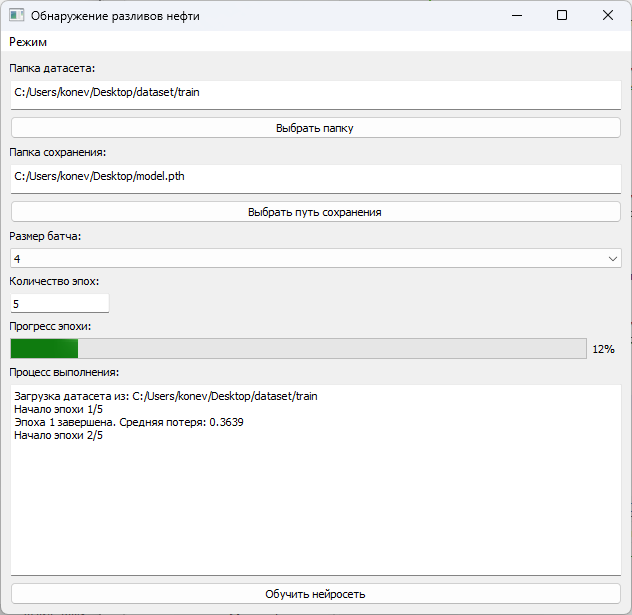
\includegraphics[width=0.7\linewidth]{images/обучение}
	\caption{Процесс обучения нейронной сети}
	\label{fig:training_process}
\end{figure}
\begin{figure}[H]
	\centering
	\includegraphics[width=0.7\linewidth]{"images/обучение результат"}
	\caption{Интерфейс программы после завершения обучения}
	\label{fig:training_result}
\end{figure}
\begin{figure}[H]
	\centering
	\includegraphics[width=0.5\linewidth]{"images/сохраненная модель"}
	\caption{Файл весов модели}
	\label{fig:saved_weights}
\end{figure}

На рисунке~\ref{fig:test_ui_default} изображено окно программы в режиме "<Тестирование">.
\begin{figure}[H]
	\centering
	\includegraphics[width=0.7\linewidth]{"images/тестирование интерфейс"}
	\caption{Окно режима "<Тестирование">}
	\label{fig:test_ui_default}
\end{figure}

На рисунке~\ref{fig:test_image_select} изображено диалоговое окно выбора тестового изображения.
\begin{figure}[H]
	\centering
	\includegraphics[width=0.7\linewidth]{"images/выбор анализируемого изображения"}
	\caption{Диалоговое окно выбора тестового изображения}
	\label{fig:test_image_select}
\end{figure}

На рисунке~\ref{fig:test_model_select} изображено диалоговое окно выбора тестируемых весов.
\begin{figure}[H]
	\centering
	\includegraphics[width=0.7\linewidth]{"images/выбор тестовой модели"}
	\caption{Диалоговое окно выбора тестируемой модели}
	\label{fig:test_model_select}
\end{figure}

На рисунке~\ref{fig:test_results_show} отображены результаты тестирования выбранных весов модели нейронной сети.
\begin{figure}[H]
	\centering
	\includegraphics[width=0.7\linewidth]{"images/результаты теста"}
	\caption{Результаты тестирования}
	\label{fig:test_results_show}
\end{figure}

\subsection{Сборка программной системы}

Программные компоненты представляют собой файлы исходных кодов программной системы.

Для сборки и компиляции программной системы использовалась библиотека Pyinstaller\cite{vasiliev-python}, позволяющая упаковать все необходимые файлы в один исполняемый файл формата .exe. Данный файл может быть запущен без предварительной установки.

Интерпретация исходных кодов на языке Python выполняется встроенным в исполняемый файл интерпретатором языка и не требует отдельной установки интерпретатора и библиотек на целевую систему.

Все программные компоненты собраны в один исполняемый файл, готовый к запуску в среде Windows.
   \section*{ЗАКЛЮЧЕНИЕ}
\addcontentsline{toc}{section}{ЗАКЛЮЧЕНИЕ}

Развитие нейронных сетей и методов машинного обучения открыло широкие возможности для автоматизации задач анализа изображений. Современные технологии позволяют обрабатывать большие объемы визуальных данных и своевременно выявлять потенциальные угрозы окружающей среде.

В условиях роста количества загрязнений водоемов, вызванных разливами нефти, применение интеллектуальных систем является эффективным инструментом мониторинга. Их использование позволяет значительно облегчить процесс обнаружения и снизить его стоимость, увеличивая при этом скорость применения.

Для решения задачи распознавания пятен нефтяных разливов была разработана интеллектуальная система на основе сверточной нейронной сети архитектуры U-Net. Система реализована в виде настольного приложения с графическим интерфейсом.

Основные результаты работы:

\begin{enumerate}
\item Проведен анализ предметной области. Проведено исследование причин возникновения разливов и нейронных сетей, являющихся наиболее эффективным методом автоматического распознавания.
\item Разработана концептуальная модель интеллектуальной системы, определены основные требования к системе и аппаратному обеспечению.
\item Осуществлено проектирование интеллектуальной системы. Разработана архитектура настольного приложения и нейронной сети. Разработан пользовательский интерфейс приложения.
\item Реализована интеллектуальная система, проведено модульное и системное тестирование разработанной нейронной сети и настольного приложения.
\end{enumerate}

Все требования, объявленные в техническом задании, были полностью реализованы. Все задачи, поставленные в начале разработки проекта, были решены.

Готовый рабочий проект представлен в виде настольного приложения с графическим интерфейсом.

}\fi
\addcontentsline{toc}{section}{СПИСОК ИСПОЛЬЗОВАННЫХ ИСТОЧНИКОВ}

\begin{thebibliography}{99}

	\bibitem{spill_db}  Алексеев Д.~В. Сравнительный анализ баз данных по разливам нефти и нефтепродуктов с морских судов / Д.~В.~Алексеев, А.~А.~Лентарёв // Вестник Государственного университета морского и речного флота имени адмирала С.~О.~Макарова. — 2022. — Т.~14. — №~6. — С.~891–904. DOI:~10.21821/2309-5180-2022-14-6-891-904. — Текст: непосредственный.
    \bibitem{spill_reasons} Владимиров~В.~А. Разливы нефти: причины, масштабы, последствия // Стратегия гражданской защиты: проблемы и исследования. — 2014. — №~1. — URL: https://cyberleninka.ru/article/n/razlivy-nefti-prichiny-masshtaby-posledstviya (дата обращения: 10.05.2025). – Текст~: непосредственный.
    \bibitem{radiophoto} Клименко~С.~К., Иванов~A.~Ю., Терелева~Н.~В. Пленочные загрязнения Керченского пролива по данным пятилетнего радиолокационного мониторинга: современное состояние и основные источники // Исследование Земли из космоса. –2022. – №~3. – С.~37–54. — DOI:~10.31857/S0205961422030071. – Текст~: непосредственный.
    \bibitem{nn_history}	Горбачевская~Е.~Н., Краснов~С.~С. История развития нейронных сетей  // Вестник ВУиТ.  — 2015. — №~1 (23). — URL: https://cyberleninka.ru/article/n/istoriya-razvitiya-neyronnyh-setey (дата обращения: 11.05.2025).  – Текст~: непосредственный.
	\bibitem{perceptron}Митина~О.~А., Ломовцев~П.~П. Перцептрон в задачах бинарной классификации // НАУ. — 2021. — №~66-1. — URL: https://cyberleninka.ru/article/n/pertseptron-v-zadachah-binarnoy-klassifikatsii (дата обращения: 11.05.2025). – Текст~: непосредственный.
	\bibitem{haikin_neural} Хайкин~С. Нейронные сети: полный курс / Саймон~Хайкин; пер. с~англ. Н.~Н.~Куссуль. --- 2-е изд., испр. --- М.: Вильямс, 2018. --- 1103~с. --- ISBN~978-5-907144-22-4. --- Текст: непосредственный.
	\bibitem{rostovtsev_neural} Ростовцев~В.~С. Искусственные нейронные сети: учебник. --- 5-е изд., стер. --- СПб.: Лань, 2025. --- 216~с. --- ISBN~978-5-507-50568-5. --- Текст: непосредственный.
	\bibitem{bychkov_cnn} Бычков~А.~Г., Киселёва~Т.~В., Маслова~Е.~В. Использование сверточных нейросетей для классификации изображений // Вестник Сибирского государственного индустриального университета. --- 2022. --- №~1. --- С.~15--19. --- Текст: непосредственный.
	\bibitem{godunov_cnn} Годунов~А.~И., Баланян~С.~Т., Егоров~П.~С. Сегментация изображений и распознавание объектов на основе технологии сверточных нейронных сетей // Надежность и качество сложных систем. --- 2021. --- №~3. --- С.~71--73. --- Текст: непосредственный.
	\bibitem{fowler_uml} Фаулер~М. UML. Основы. --- 3-е изд. --- СПб.: Символ-Плюс, 2015. --- 192~с. --- ISBN~978-5-93286-060-1. --- Текст: непосредственный.
	\bibitem{lutz_python1} Лутц~М. Изучаем Python. Том~1: учебное пособие / М.~Лутц. --- 5-е изд. --- М.: Вильямс, 2020. --- 832~с. --- ISBN~978-5-907144-52-1. --- Текст: непосредственный.
	\bibitem{chollet_python} Шолле~Ф. Глубокое обучение на Python / пер. с~англ. --- М.: ДМК~Пресс, 2018. --- 384~с. --- ISBN~978-5-4461-0770-4. --- Текст: непосредственный.
	\bibitem{lutz_python2} Лутц~М. Изучаем Python. Том~2 / М.~Лутц. --- 5-е изд. --- М.: Вильямс, 2020. --- 720~с. --- ISBN~978-5-907144-53-8. --- Текст: непосредственный.
	\bibitem{pointer_pytorch} Пойнтер~Я. Программируем с~PyTorch: создание приложений глубокого обучения. --- СПб.: Питер, 2020. --- 256~с. --- ISBN~978-5-4461-1677-5. --- Текст: непосредственный.
	\bibitem{bender_python} Бендер~Д. Python для анализа данных. --- М.: ДМК~Пресс, 2015. --- 482~с. --- ISBN~978-5-97060-315-4. --- Текст: непосредственный.
	\bibitem{halyapin_uml} Халяпин~Д.~Б. UML. Проектирование систем реального времени, параллельных и распределенных приложений / Д.~Б.~Халяпин. --- Москва: Озон, 2023. --- 352~с. --- ISBN~978-5-6048804-3-2. --- Текст: непосредственный.
	\bibitem{sorokin_cnn} Сорокин~А.~Б., Железняк~Л.~М., Зикеева~Е.~А. Сверточные нейронные сети: примеры реализаций: учебное пособие. --- М.: МИРЭА, 2020. --- 1~электрон. опт. диск (CD-ROM). --- Текст: непосредственный.
	\bibitem{mueller_brockmann} Мюллер-Брокманн~Й. Модульные системы в графическом дизайне. --- М.: Студия Артемия Лебедева, 2018. --- 176~с. --- ISBN~978-5-98062-140-7. --- Текст: непосредственный.
	\bibitem{hillard-packaging} Хиллард~Д. Публикация пакетов Python. Тестирование, распространение и автоматизация проектов. — М.: Бомбора, 2024. — 288с. — ISBN~978-5-04-189146-6. — Текст: непосредственный.
	\bibitem{vasiliev-python} Васильев~А.~Н. Программирование на~Python в~примерах и~задачах. — М.: Бомбора, 2021. — 384~с. — ISBN~978-5-04-103199-2. — Текст: непосредственный.
\end{thebibliography}

\ifВКР{\appendix{Представление графического материала}

Графический материал, выполненный на отдельных листах,
изображен на рисунках А.1--А.\arabic{числоПлакатов}.
\setcounter{числоПлакатов}{0}

\renewcommand{\thefigure}{А.\arabic{figure}} % шаблон номера для плакатов

\begin{landscape}

\begin{плакат}
    
\includegraphics[width=0.82\linewidth]{титульник.eps}
    \заголовок{Сведения о ВКРБ}
    \label{pl1:image}      
\end{плакат}

\begin{плакат}
	
\includegraphics[width=0.82\linewidth]{актуальность.eps}
	\заголовок{Актуальность проблемы}
	\label{pl12:image}      
\end{плакат}

\begin{плакат}
	
\includegraphics[width=0.82\linewidth]{цель и задачи.eps}
	\заголовок{Цель и задачи работы}
	\label{pl2:image}      
\end{плакат}

\begin{плакат}
	
\includegraphics[width=0.82\linewidth]{диаграмма прецедентов.eps}
	\заголовок{Диаграмма прецедентов}
	\label{pl3:image}      
\end{плакат}

\begin{плакат}
	
\includegraphics[width=0.82\linewidth]{архитектура системы.eps}
	\заголовок{Архитектура интеллектуальной системы}
	\label{pl4:image}      
\end{плакат}

\begin{плакат}
	
\includegraphics[width=0.82\linewidth]{архитектура сети.eps}
	\заголовок{Архитектура нейронной сети}
	\label{pl5:image}      
\end{плакат}

\begin{плакат}
	
\includegraphics[width=0.82\linewidth]{обучение нейросети.eps}
	\заголовок{Обучение нейронной сети}
	\label{pl6:image}      
\end{плакат}

\begin{плакат}
	
\includegraphics[width=0.82\linewidth]{интерфейс анализ.eps}
	\заголовок{Окно анализа изображения}
	\label{pl7:image}      
\end{плакат}

\begin{плакат}
	
\includegraphics[width=0.82\linewidth]{интерфейс обучение.eps}
	\заголовок{Окно обучения нейронной сети}
	\label{pl8:image}      
\end{плакат}

\begin{плакат}
	
\includegraphics[width=0.82\linewidth]{интерфейс тестирование.eps}
	\заголовок{Окно тестирования нейронной сети}
	\label{pl9:image}      
\end{плакат}

\begin{плакат}
	
\includegraphics[width=0.82\linewidth]{результаты тестирования сети.eps}
	\заголовок{Тестирование обученной нейронной сети}
	\label{pl10:image}      
\end{плакат}

\begin{плакат}
	
\includegraphics[width=0.82\linewidth]{результаты тестирования 2.eps}
	\заголовок{Тестирование обученной нейронной сети}
	\label{pl13:image}      
\end{плакат}

\begin{плакат}
	
\includegraphics[width=0.82\linewidth]{заключение.eps}
	\заголовок{Заключение}
	\label{pl11:image}      
\end{плакат}

\end{landscape}
}\fi
\ifПрактика{}\else{\appendix{Фрагменты исходного кода программы}

main.tex
\lstinputlisting[language=Tex, frame=none]{main.tex}

ТехПроект.tex
\lstinputlisting[language=Tex, frame=none]{ТехПроект.tex}

\ifВКР{
\newpage
\addcontentsline{toc}{section}{На отдельных листах (CD-RW в прикрепленном конверте)}
\noindent
\begin{tabular}{p{5.8cm}C{4.8cm}C{4.8cm}}
   Автор ВКР & \lhrulefill{\fill} & \fillcenter\Автор \\
            \setarstrut{\footnotesize}
           & \footnotesize{(подпись, дата)} & \\
            \restorearstrut
   Руководитель ВКР & \lhrulefill{\fill} & \fillcenter\Руководитель \\
            \setarstrut{\footnotesize}
           & \footnotesize{(подпись, дата)} & \\
            \restorearstrut
   Нормоконтроль & \lhrulefill{\fill} & \fillcenter\Нормоконтроль \\
            \setarstrut{\footnotesize}
           & \footnotesize{(подпись, дата)} & \\
            \restorearstrut
\end{tabular}
\vskip 2cm
\begin{center}
\textbf{Место для диска}
\end{center}
}\fi
}\fi
\end{document}
